\chapter{Especificação e Arquitetura} \label{cap:especificacao}

O presente capítulo apresentará os componentes da arquitetura do sistema, bem como o detalhamento das responsabilidades de cada um.

\section{Visão Geral}
\subsection{Componentes e Responsabilidades}

A utilização de LESC e HTTPS na comunicação não é suficiente para prover os serviços de segurança necessários para o funcionamento desejado do sistema. Esses dois mecanismos garantem
segurança na comunicação entre dongle e app e entre app e servidor, respectivamente, mas não conseguem garantir que pacotes realmente foram gerados pelo dongle, uma vez que eles
serão transmitidos por meio de um intermediário que tem controle total sobre o conteúdo.

\subsection{Fluxo de Dados fim a fim}
\subsection{Decisão do Método de Autenticação}

O \textit{dongle} deverá tratar os dados gerados de modo que o servidor, ao recebê-los, consiga verificar a autenticidade e a integridade dos dados recebidos. Para isso, se apresentam duas opções: a utilização de MAC (Message Authentication Code) com chave simétrica pré-compartilhada (PSK) ou a utilização de assinaturas digitais via chave assimétrica.

A escolha entre as duas opções se dará pela realização de testes de desempenho (TODO: DIZER O QUE FOI RESOLVIDO E APONTAR PARA SEÇÃO EM QUE HAVERÁ A DESCRIÇÃO DO BENCHMARK.)

Na abordagem com assinatura digital, cada bloco de dados gravado na flash do dongle passa a ser autenticado com ECDSA sobre a curva P-256 (secp256r1 ), usando SHA-256 como função de hash, em lugar da tag HMAC-SHA256 calculada com Krec. Na fabricação, o dongle gera um par de chaves. A chave privada fica protegida na NVS cifrada e é usada para assinar cada bloco. A chave pública é registrada no servidor, que a usa apenas para verificar as assinaturas dos blocos recebidos. Para evitar que um nonce mal gerado comprometa a chave privada, as assinaturas são geradas de forma determinística, conforme a RFC 6979.

A principal vantagem da assinatura em relação ao HMAC é que o servidor guarda somente a chave pública, de modo que nem um invasor com acesso ao servidor consegue forjar blocos válidos. Além disso, a chave privada garante irretratabilidade para o motorista, não sendo possível forjar dados no seu nome sem a obtenção da chave privada, e isso pode ser importante para algumas aplicações como seguros personalizados. Escolheu-se ECDSA em vez de RSA por oferecer segurança equivalente com chaves e assinaturas muito menores: uma assinatura de 64 bytes, próxima da tag HMAC de 32 bytes, em vez dos 256 bytes do RSA-2048. A curva P-256 foi escolhida por ser a mesma que o LESC usa no pareamento BLE, por estar disponível no mbedTLS do ESP32, por ter aceleração em hardware nos modelos mais recentes da Espressif e por ser a única curva suportada pelo elemento seguro ATECC608B, previsto como evolução do projeto. Ela também é amplamente suportada pelas ferramentas do servidor, como a biblioteca padrão do Go e o HashiCorp Vault.

\section{Contratos de Dados}
\subsection{Enquadramento e Fragmentação}


Os comandos ELM327, incluindo os comandos customizados de configuração definidos no projeto, são enviados do app para o dongle a partir 
do serviço NUS. Enquanto isso, os comandos de handshake e envio de blocos passam por um outro serviço criado para o projeto, chamado 
SYNC. Assim como o NUS, o SYNC expõe uma característica RX, na qual o dongle recebe dados do app, e uma característica TX, na qual 
o dongle envia dados para o app; no entanto, enquanto o NUS recebe texto, o serviço SYNC envia e recebe dados binários. Com essa separação,
cada fluxo de dados entre app e dongle fica separado e com suas próprias responsabilidades, ajudando na remontagem de blocos a partir dos fragmentos.


Além dos tipos de blocos definidos no handshake, existem mais alguns tipos que precisam ser usados para orquestrar a comunicação entre app e dongle, sendo
todos eles apresentados na tabela \ref{table:tipos-blocos}. Quando são enviados via BLE no SYNC\_RX, como convenção do projeto, os blocos são estruturados no formato TLV (type, length, value), 
sendo 3 bytes concatenados no início de cada bloco, o primeiro byre representa o tipo e os outros dois o comprimento do corpo da mensagem, ou seja, sem contar o tipo e comprimento. Além disso, quando são
enviados no SYNC\_TX, também é necessário englobar o bloco TLV em um enquadramento com um byte de controle na frente: nesse byte de controle, o bit 7 vale 1 quando for um início de mensagem e os bits de 6 a 0
servem de contador de modo que o primeiro fragmento da mensagem completa começa em 0 e a cada fragmento vai somando 1 até 127, voltando para 0 no próximo fragmento, o que permite detectar fragmentos faltantes.
Para remontar, então, basta desencapsular e juntar os fragmentos na ordem correta até o comprimento marcado ser alcançado.
Isso é necessário pelo fato de as mensagens do SYNC\_TX poderem ser fragmentadas em vários pacotes BLE. O formato do pacote de cada característica do SYNC pode ser visto na figura \ref{fig:sync-tvl}.

\begin{figure}[H]
	\centering
	\caption{Formato dos dados nas características RX e TX do serviço SYNC}
	\label{fig:sync-tvl}
	\begin{tikzpicture}[
		campo/.style={draw, minimum height=0.9cm, inner sep=1pt, font=\small, align=center},
		controle/.style={campo, fill=orange!40},
		ponteiro/.style={-{Stealth[length=2.5mm]}, thick},
		rotulo/.style={align=center, font=\small, anchor=north},
		chave/.style={decorate, decoration={brace, amplitude=5pt}, thick},
		titulo/.style={font=\small\bfseries, anchor=south west}
	]
		% \campo{x}{y}{largura}{texto}{estilo}{id}
		\newcommand{\campo}[6]{\node[#5, anchor=north west, minimum width=#3 cm] (#6) at (#1,#2) {#4};}
		% \seta{id}{texto}
		\newcommand{\seta}[2]{\draw[ponteiro] ([yshift=-0.9cm]#1.south) -- (#1.south);
			\node[rotulo] at ([yshift=-0.9cm]#1.south) {#2};}

		% SYNC_RX: formato TLV
		\node[titulo] at (0,0.2) {SYNC\_RX};
		\campo{0}{0}{1.8}{T\\(1 byte)}{campo}{rt}
		\campo{1.8}{0}{1.8}{L\\(2 bytes)}{campo}{rl}
		\campo{3.6}{0}{5.4}{V $\cdots$\\($n$ bytes)}{campo}{rv}
		\seta{rt}{tipo}
		\seta{rl}{comprimento}
		\seta{rv}{valor}

		% SYNC_TX: TLV precedido por um byte de controle
		\node[titulo] at (0,-3.1) {SYNC\_TX};
		% byte de controle: 8 bits, apenas o primeiro (bit de controle) é destacado
		\campo{0}{-4.4}{0.3}{\tiny 7}{controle}{tc}
		\foreach \i/\b in {1/6,2/5,3/4,4/3,5/2,6/1,7/0} {
			\node[campo, fill=orange!15, anchor=north west, minimum width=0.3cm, font=\tiny] at (0.3*\i,-4.4) {\b};
		}
		\node[coordinate] (contini) at (0.3,-5.3) {};
			\node[coordinate] (contfim) at (2.4,-5.3) {};
			\draw[chave, decoration={brace, mirror, amplitude=5pt}] (contini) -- (contfim)
				node[rotulo, midway, anchor=north, yshift=-7pt, xshift=0.5cm] {contador\\(bits 6 a 0)};
			\node[coordinate] (cini) at (0,-4.4) {};
		\node[coordinate] (cfim) at (2.4,-4.4) {};
		\draw[chave] ([yshift=3pt]cini) -- ([yshift=3pt]cfim)
			node[rotulo, midway, anchor=south, yshift=7pt] {byte de controle (C, 1 byte)};
		\campo{2.4}{-4.4}{1.8}{T\\(1 byte)}{campo}{tt}
		\campo{4.2}{-4.4}{1.8}{L\\(2 bytes)}{campo}{tl}
		\campo{6.0}{-4.4}{5.4}{V $\cdots$\\($n$ bytes)}{campo}{tv}
		\seta{tc}{bit 7\\(controle)}
		\seta{tt}{tipo}
		\seta{tl}{comprimento}
		\seta{tv}{valor}
	\end{tikzpicture}
	\legend{Fonte: elaborado pelo autor.}
\end{figure}


\subsection{Estrutura dos Blocos e dos Registros}


Os blocos marcadores BOOT e LOSS, usados para declarar lacunas na sequência (seção \ref{subsec:riscos-sincronizacao}), são blocos 0x03 e são tratados pelo app exatamente como blocos de dados: o app
não os distingue de um bloco com leituras de PID. Seguindo a convenção do registro de GPS (tipo 0xFF), são reservados os tipos de registro 0xFE (BOOT) e 0xFD (LOSS), ambos no formato tipo (1) $\mid$
$\Delta t$ (2) $\mid$ $from\_seq$ (4) $\mid$ $to\_seq$ (4), com 11 bytes; com o cabeçalho de 12 bytes, o bloco marcador tem 23 bytes de conteúdo, mais a tag de 32 bytes. Por serem blocos 0x03, os
marcadores ocupam um $seq$, recebem a tag $K_{rec}$ da equação \ref{eq:hmac-sha256-rec} e percorrem o mesmo fluxo dos blocos de dados: são contados no $HEAD_{seq}$, pedidos via Pedido de lote 0x05,
fragmentados no SYNC\_TX, enviados no \texttt{POST /v1/dongles/blocos} e confirmados pelo ACK 0x04. Como o marcador faz parte do conteúdo autenticado, o app não consegue forjar um LOSS nem
transformar um bloco de dados em marcador.

Quando o dongle dá flush em um bloco para a \textit{flash}, ele envia um aviso de novo bloco (0x07) para o app. Quando esse aviso chega, caso o app já tenha disponível um valor de $ACK_{seq}$ válido, ele calcula o valor de quantos blocos estão pendentes de envio a partir de $HEAD_{seq} - ACK_{seq}$, sendo o $HEAD_{seq}$ recebido via aviso. As flags desse bloco de aviso podem ser vistas na tabela \ref{tab:flags-aviso-novo-bloco}. Caso o app ainda não tenha um handshake válido, o dongle solicita para o app que faça um pedido de desafio para o servidor, iniciando o processo de handshake.

É importante notar que o MTU do BLE não suporta um bloco inteiro, que fica negociado em torno de 272 bytes. O bloco completo, como mostra a figura \ref{fig:bloco-completo} terá 1059 bytes, sendo 1 byte com o 
tipo, 2 bytes com o comprimento, 1024 bytes de dados e, por fim, 32 bytes de tag. Os bytes do CRC são conferidos antes de o dongle enviar os blocos via BLE, então não aparecem aqui.

A figura \ref{fig:bloco-completo} mostra o bloco já pronto para a transmissão, enquanto o que é diferente do que fica gravado na \textit{flash} , como mostra a figura \ref{fig:bloco-flash}. O bloco salvo não tem o
envelope de tipo e comprimento, que é só uma convenção para o enquadramento no SYNC\_RX e é montado na hora de enviar; em compensação, tem mais 4 bytes de CRC32 no final, calculados sobre os dados e a tag
(seção \ref{subsec:riscos-sincronizacao}), usados para detectar corrompimento antes do envio. Para montar o bloco da figura \ref{fig:bloco-completo} a partir do que está na flash, o dongle então descarta
o CRC já verificado e acrescenta o envelope TLV com tipo 0x03 e o comprimento.


\begin{figure}[H]
	\centering
	\caption{Estrutura do bloco como gravado na \textit{flash}}
	\label{fig:bloco-flash}
	\begin{tikzpicture}[
		campo/.style={draw, minimum height=0.9cm, inner sep=1pt, font=\small, align=center},
		posini/.style={font=\scriptsize, anchor=north west, inner sep=1pt},
		posfim/.style={font=\scriptsize, anchor=north east, inner sep=1pt},
		titulo/.style={font=\small\bfseries, anchor=south west}
	]
		% \campo{x}{y}{largura}{texto}{posição inicial}
		\newcommand{\campo}[5]{%
			\node[campo, anchor=north west, minimum width=#3 cm] at (#1,#2) {#4};
			\node[posini] at (#1,#2-0.9) {#5};}
		% \fim{x}{y}{posição final}
		\newcommand{\fim}[3]{\node[posfim] at (#1,#2-0.9) {#3};}

		\node[titulo] at (0,0.2) {Bloco na \textit{flash} (até 1060 bytes)};
		\campo{0}{0}{6.6}{dados\\(1024 bytes, cabeçalho + registros) $\cdots$}{0}
		\campo{6.6}{0}{3.4}{$tag$ ($K_{rec}$)\\(32 bytes)}{1024}
		\campo{10.0}{0}{1.6}{CRC32\\(4 bytes)}{1056}
		\fim{11.6}{0}{1060}
	\end{tikzpicture}
	\legend{Fonte: elaborado pelo autor.}
\end{figure}



\begin{figure}[H]
	\centering
	\caption{Estrutura do bloco completo de dados}
	\label{fig:bloco-completo}
	\begin{tikzpicture}[
		campo/.style={draw, minimum height=0.9cm, inner sep=1pt, font=\small, align=center},
		posini/.style={font=\scriptsize, anchor=north west, inner sep=1pt},
		posfim/.style={font=\scriptsize, anchor=north east, inner sep=1pt},
		titulo/.style={font=\small\bfseries, anchor=south west}
	]
		% \campo{x}{y}{largura}{texto}{posição inicial}
		\newcommand{\campo}[5]{%
			\node[campo, anchor=north west, minimum width=#3 cm] at (#1,#2) {#4};
			\node[posini] at (#1,#2-0.9) {#5};}
		% \fim{x}{y}{posição final}
		\newcommand{\fim}[3]{\node[posfim] at (#1,#2-0.9) {#3};}

		\node[titulo] at (0,0.2) {Bloco: 0x03 (1059 bytes)};
		\campo{0}{0}{1.8}{tipo\\(1 byte)}{0}
		\campo{1.8}{0}{2.8}{comprimento\\(2 bytes)}{1}
		\campo{4.6}{0}{5.4}{dados\\(1024 bytes) $\cdots$}{3}
		\campo{10.0}{0}{3.4}{$tag$ ($K_{rec}$)\\(32 bytes)}{1027}
		\fim{13.4}{0}{1059}
	\end{tikzpicture}
	\legend{Fonte: elaborado pelo autor.}
\end{figure}


A área de dados do bloco (figura \ref{fig:bloco-completo}), de até 1024 bytes, não é só registros: como mostra a figura \ref{fig:divisao-dados-bloco}, ela começa com o cabeçalho de 12 bytes do próprio
bloco, composto por $seq$ (4 bytes), $boot\_id$ (2 bytes), $t_{ms}$ inicial (4 bytes) e \textit{tamanho} (2 bytes), e só depois vêm os registros, em até 1012 bytes. É nesse cabeçalho que $seq$ fica: ele não é um
registro de medida, é o identificador de posição do bloco na sequência, usado para contar $HEAD_{seq}$ e para ordenar e detectar lacunas no servidor.

Os registros que seguem o cabeçalho são concatenados até o limite indicado pelo próprio campo \textit{tamanho}. Todo registro começa com \textit{tipo} (1 byte) e $\Delta t$ (2 bytes, deslocamento em
milissegundos a partir do $t_{ms}$ inicial do cabeçalho); o restante depende do \textit{tipo}. No caso de medida, cada leitura de PID ocupa 5 bytes (\textit{tipo}, $\Delta t$ e valor) e cada posição GPS
ocupa 15 bytes (\textit{tipo} 0xFF, $\Delta t$, latitude, longitude e altitude), e os registros se repetem até o bloco ser fechado. No caso de marcador, o bloco carrega um único registro de 11 bytes no
lugar das leituras: BOOT (\textit{tipo} 0xFE) ou LOSS (\textit{tipo} 0xFD), com $from\_seq$ e $to\_seq$ em vez do valor medido; o restante da área de 1024 bytes simplesmente não é escrito, pois o
\textit{tamanho} do bloco reflete só os 12 bytes do cabeçalho mais os 11 bytes do registro (seção \ref{sec:app-ble-dongle}).

\begin{figure}[H]
	\centering
	\caption{Divisão dos 1024 bytes da área de dados: cabeçalho do bloco e registros}
	\label{fig:divisao-dados-bloco}
	\begin{tikzpicture}[
		campo/.style={draw, minimum height=0.9cm, inner sep=1pt, font=\small, align=center},
		cabecalho/.style={campo, fill=blue!15},
		registros/.style={campo, fill=orange!20},
		posini/.style={font=\scriptsize, anchor=north west, inner sep=1pt},
		posfim/.style={font=\scriptsize, anchor=north east, inner sep=1pt},
		titulo/.style={font=\small\bfseries, anchor=south west}
	]
		% \campo{x}{y}{largura}{texto}{estilo}{posição inicial}
		\newcommand{\campo}[6]{%
			\node[#5, anchor=north west, minimum width=#3 cm] at (#1,#2) {#4};
			\node[posini] at (#1,#2-0.9) {#6};}
		% \fim{x}{y}{posição final}
		\newcommand{\fim}[3]{\node[posfim] at (#1,#2-0.9) {#3};}

		\node[titulo] at (0,0.2) {Área de dados do bloco 0x03 (1024 bytes)};
		\campo{0}{0}{1.4}{$seq$}{cabecalho}{0}
		\campo{1.4}{0}{1.4}{$boot_{id}$}{cabecalho}{4}
		\campo{2.8}{0}{1.6}{$t_{ms}$ inicial}{cabecalho}{6}
		\campo{4.4}{0}{1.6}{tamanho}{cabecalho}{10}
		\campo{6.0}{0}{5.4}{registros $\cdots$\\(até 1012 bytes)}{registros}{12}
		\fim{11.4}{0}{1024}

		\draw[decorate, decoration={brace, amplitude=6pt, mirror}, thick]
			(0,-1.3) -- (6.0-0.05,-1.3)
			node[midway, below=6pt, align=center, font=\footnotesize] {cabeçalho do bloco\\(12 bytes)};
		\draw[decorate, decoration={brace, amplitude=6pt, mirror}, thick]
			(6.0+0.05,-1.3) -- (11.4,-1.3)
			node[midway, below=6pt, align=center, font=\footnotesize] {registros de medida\\ou registro marcador};
	\end{tikzpicture}
	\legend{Fonte: elaborado pelo autor.}
\end{figure}


\begin{figure}[H]
	\centering
	\caption{Estrutura dos registros na área de dados: casos de medida e de marcador}
	\label{fig:registros-dados-bloco}
	\begin{tikzpicture}[
		campo/.style={draw, minimum height=0.9cm, inner sep=1pt, font=\small, align=center},
		posini/.style={font=\scriptsize, anchor=north west, inner sep=1pt},
		posfim/.style={font=\scriptsize, anchor=north east, inner sep=1pt},
		titulo/.style={font=\small\bfseries, anchor=south west}
	]
		% \campo{x}{y}{largura}{texto}{posição inicial}
		\newcommand{\campo}[5]{%
			\node[campo, anchor=north west, minimum width=#3 cm] at (#1,#2) {#4};
			\node[posini] at (#1,#2-0.9) {#5};}
		% \fim{x}{y}{posição final}
		\newcommand{\fim}[3]{\node[posfim] at (#1,#2-0.9) {#3};}

		% Leitura de PID (caso de medida)
		\node[titulo] at (0,0.2) {Leitura de PID (5 bytes)};
		\campo{0}{0}{1.4}{tipo\\(PID)}{0}
		\campo{1.4}{0}{1.6}{$\Delta t$}{1}
		\campo{3.0}{0}{1.4}{valor}{3}
		\fim{4.4}{0}{5}

		% Posição GPS (caso de medida)
		\node[titulo] at (0,-2.4) {Posição GPS (15 bytes, tipo 0xFF)};
		\campo{0}{-2.4}{1.4}{0xFF}{0}
		\campo{1.4}{-2.4}{1.6}{$\Delta t$}{1}
		\campo{3.0}{-2.4}{1.4}{lat}{3}
		\campo{4.4}{-2.4}{1.4}{lon}{7}
		\campo{5.8}{-2.4}{1.4}{alt}{11}
		\fim{7.2}{-2.4}{15}

		% Marcador BOOT/LOSS (caso de marcador)
		\node[titulo] at (0,-4.8) {Marcador: BOOT (0xFE) ou LOSS (0xFD) -- 11 bytes};
		\campo{0}{-4.8}{1.4}{tipo}{0}
		\campo{1.4}{-4.8}{1.6}{$\Delta t$}{1}
		\campo{3.0}{-4.8}{1.8}{$from_{seq}$}{3}
		\campo{4.8}{-4.8}{1.8}{$to_{seq}$}{7}
		\fim{6.6}{-4.8}{11}
	\end{tikzpicture}
	\legend{Fonte: elaborado pelo autor.}
\end{figure}




\subsection{Mensagens de Handshake}


Assim que há um pedido de handshake do dongle ou assim que o app se conecta com a internet, o \textit{handshake}, utilizando os parâmetros definidos na tabela \ref{table:params-handshake},
começa e segue a seguinte sequência de passos, abstraindo a intermediação do app:

\begin{enumerate}
	\item Dongle pede que $S_{App}$ envie um desafio
	\item Server anota $S1$
	\item Server envia um bloco desafio tipo 0x01 para o dongle contendo: $c_S$, $N_S$, $ACK_{seq}$, $c_{conf}$, $flags_c$, $diag_min$ e $tag$ (47 bytes) com destino ao dongle
	\item Dongle responde um bloco tipo 0x02 contendo: $c_S$, $N_S$, $TAIL_{seq}$, $HEAD_{seq}$, $boot\_id$, $t_{ms}$ e $tag$ (50 bytes) com destino ao server
	\item Com $S2$, o server fecha a âncora de tempo para $boot\_id$ segundo algoritmo de Cristian e, com $TAIL_{seq}$, verifica se houve descarte por \textit{flash} cheia, atualizando $ACK_{seq}$
	(seção \ref{subsec:riscos-sincronizacao})
	\item Server envia bloco ACK tipo 0x04 contendo: $ACK_{seq}$, $c_{conf}$, $flags_a$, e $tag$ (25 bytes) com destino ao dongle
	\item Server envia, com destino ao app, um token JWT válido para receber blocos do app.
\end{enumerate}

\begin{figure}[H]
	\centering
	\caption{Diagrama de sequência do \textit{handshake} e da âncora de tempo}
	\label{fig:sequencia-handshake}
	% Fonte PlantUML: ../assets/aux-docs/plantuml/handshake-sequencia.puml
	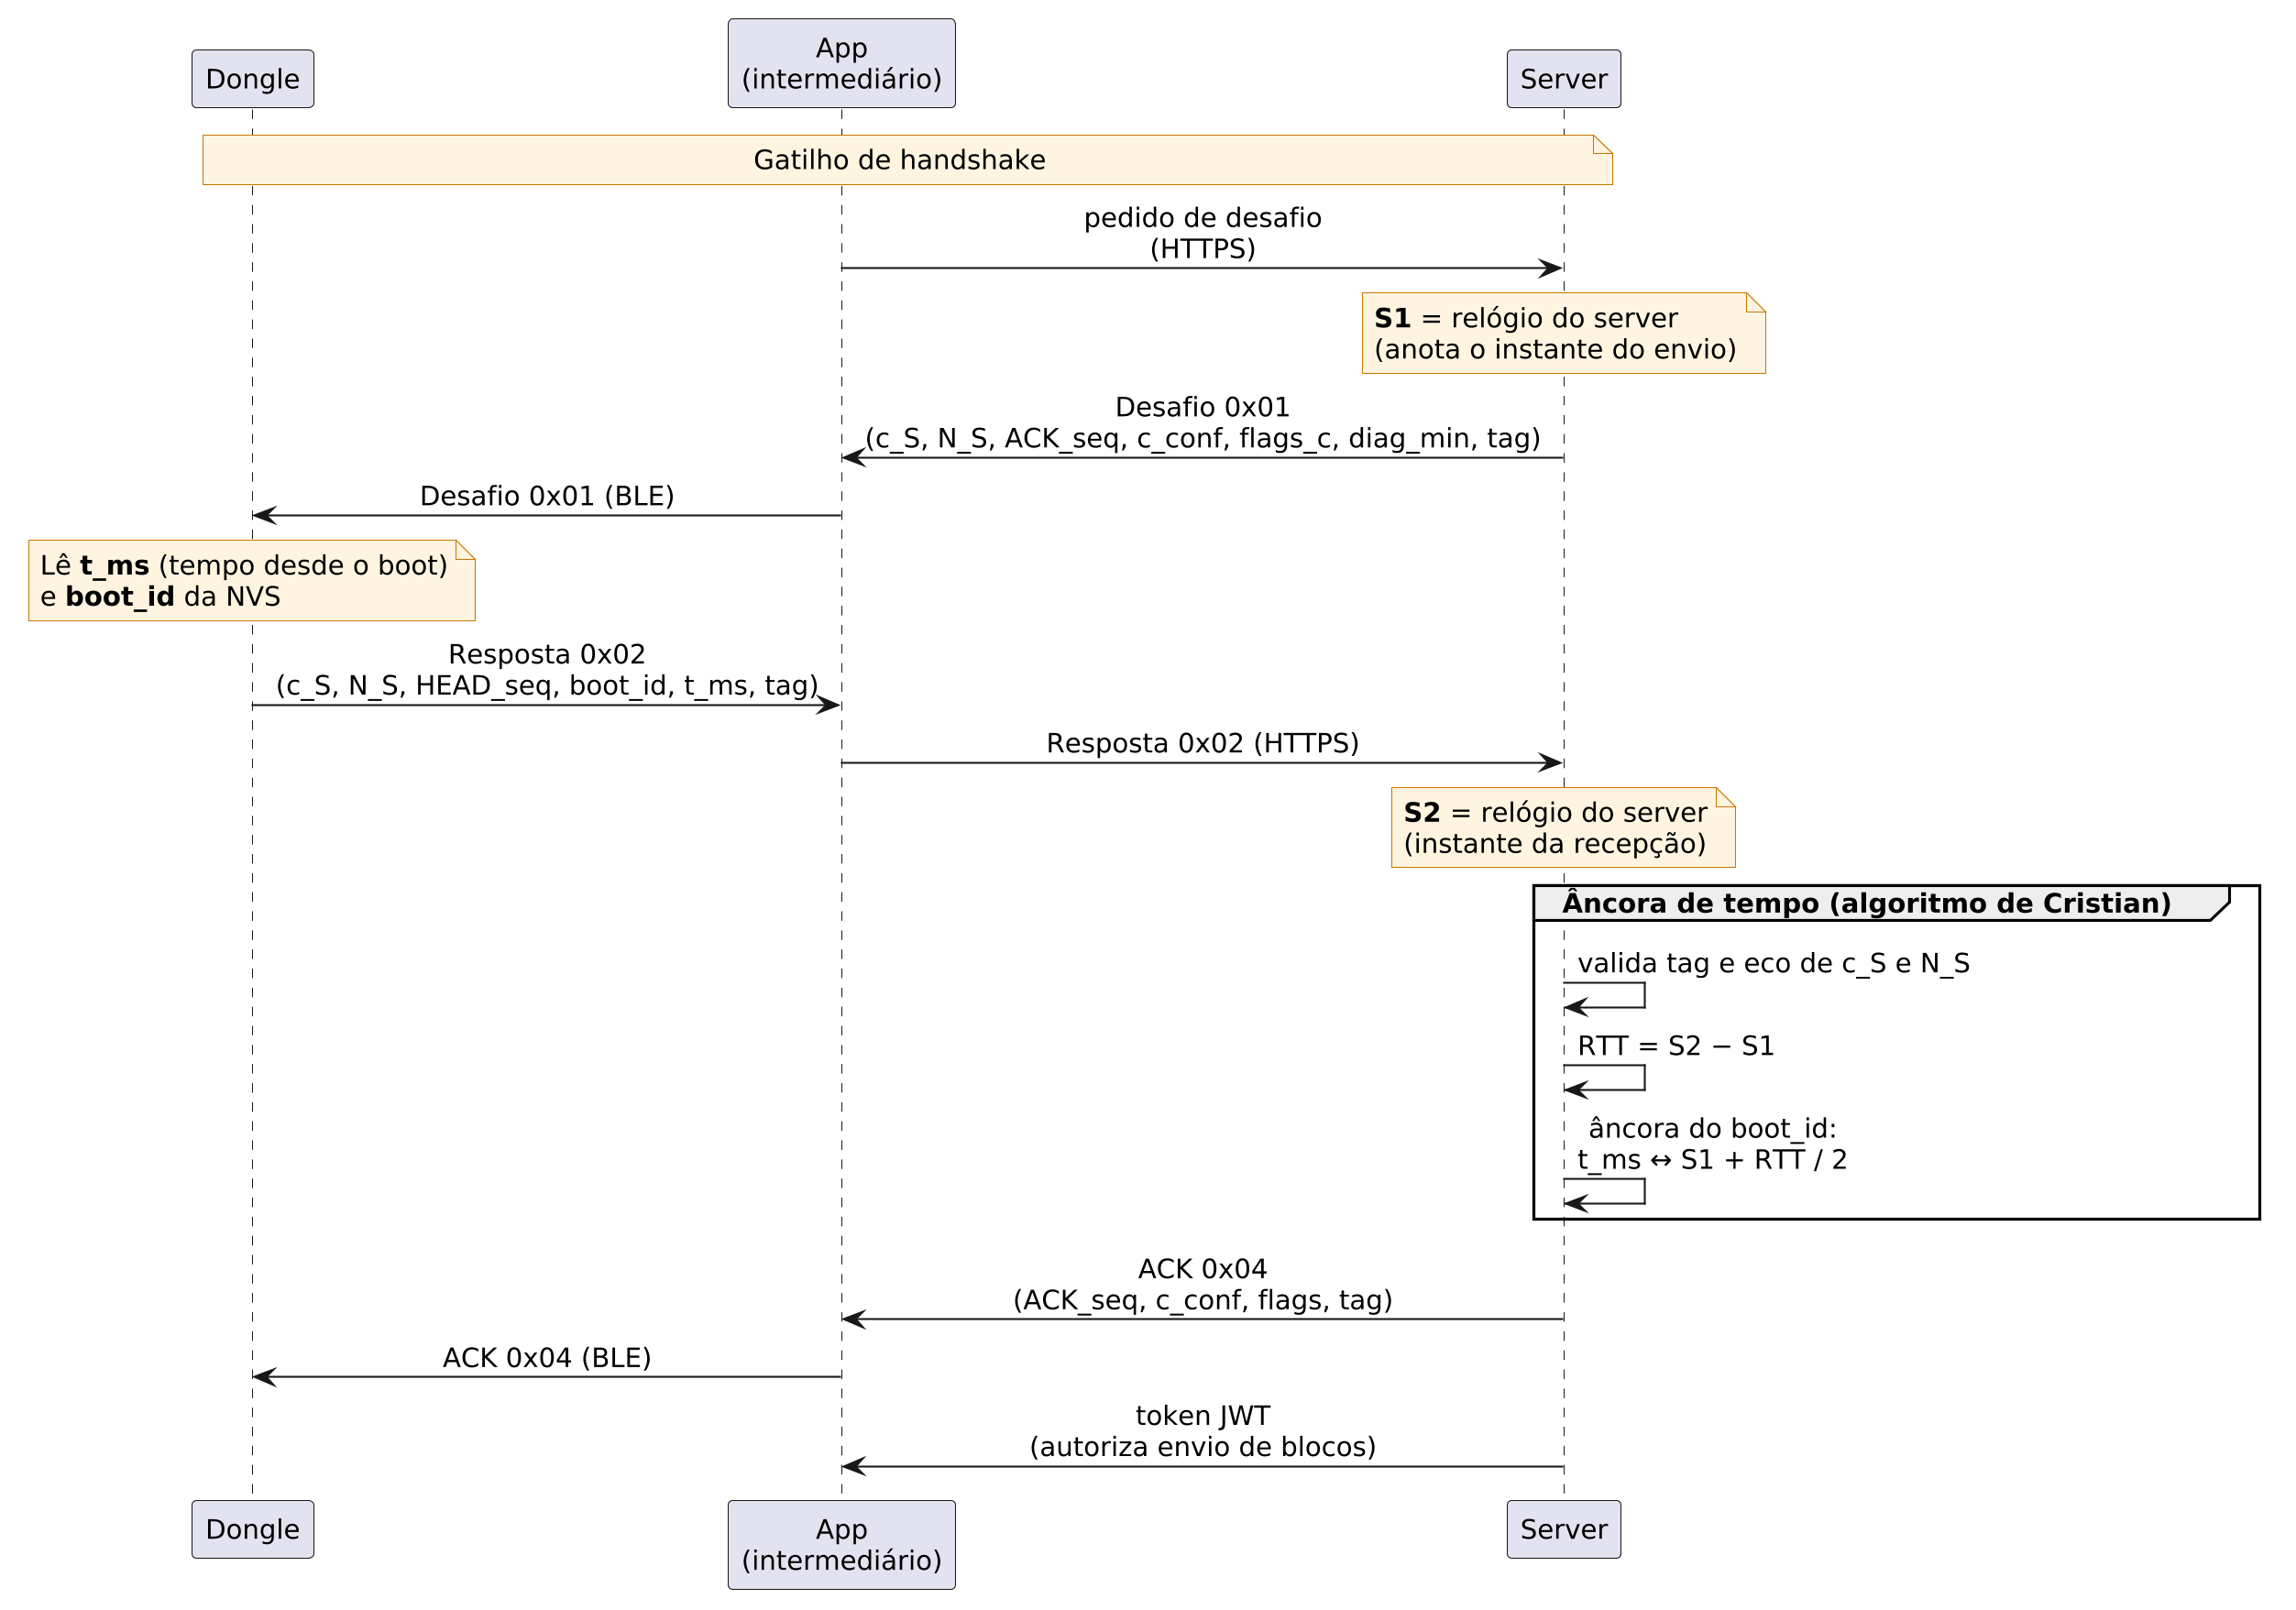
\includegraphics[width=\textwidth]{assets/cap7-especificacao/handshake-sequencia.png}
	\legend{Fonte: elaborado pelo autor.}
\end{figure}


\begin{table}[H]
	\centering
	\caption{Parâmetros do processo de \textit{handshake}}
	\label{table:params-handshake}
	\begin{tabular}{|>{\centering\arraybackslash}m{0.15\textwidth}|>{\raggedright\arraybackslash}m{0.45\textwidth}|>{\centering\arraybackslash}m{0.15\textwidth}|>{\centering\arraybackslash}m{0.1\textwidth}|}
		\hline
		\textbf{Parâmetro} & \textbf{Descrição} & \textbf{Origem} & \textbf{Bytes} \\
		\hline
		$c_{S}$ & Contador de desafios associado ao dongle pelo seu \textit{DevId} & $S_{App}$ & 4 \\
		\hline
		$N_{S}$ & \textit{Nonce} que identifica o desafio & $S_{App}$ & 16 \\
		\hline
		$ACK_{seq}$ & Fronteira que indica o último \textit{seq} recebido pelo server & $S_{App}$ & 4 \\
		\hline
		$c_{conf}$ & $c_{S}$ do último desafio aceito para conferência & $S_{App}$ & 4 \\
		\hline
		$flags_c$ & Bit 0: indica se ativa modo diagnóstico; Outros bits reservados & $S_{App}$ & 1 \\
		\hline
		$diag_min$ & Tempo em minutos que o dispositivo ficará em modo diagnóstico & $S_{App}$ & 2 \\
		\hline
		$TAIL_{seq}$ & Valor de $seq$ do bloco mais antigo ainda na \textit{flash}; $HEAD_{seq} + 1$ se a \textit{flash} está vazia & Dongle & 4 \\
		\hline
		$HEAD_seq$ & Valor de $seq$ do último bloco gravado no LittleFS & Dongle & 4 \\
		\hline
		$boot\_id$ & O valor de ID do \textit{boot} atual do dongle & Dongle & 2 \\
		\hline
		$t_{ms}$ & Tempo em milissegundos desde o boot no instante da resposta & Dongle & 4 \\
		\hline
		$flags_a$ & Bit 0: indica falha na sincronização de tempo, \textit{handshake} deve ser repetido; Outros bits reservados & $S_{App}$ & 1 \\
		\hline
		$tag$ & Tag calculada via HMAC-SHA256 & Dongle ou $S_{App}$ & 16 \\
		\hline
	\end{tabular}
\end{table}


Para o cálculo da tag das mensagens de handshake, que são relacionadas à autenticação, é usada a chave $K_{auth}$ para gerar o HMAC-SHA256 segundo a 
equação \ref{eq:hmac-sha256-auth}, que é truncado em seguida para 16 bytes a fim de economizar banda na transmissão. Aqui é possível truncar devido ao 
ato de o server ter permissão de gerar MACs com $K_{auth}$ no KMS, o que possibilita o servidor gerar o HMAC e comparar os primeiros 16 bytes; como o server 
não consegue gerar HMAC para $K_{rec}$, não é possível truncar o HMAC dos blocos, mostrado na equação \ref{eq:hmac-sha256-rec}, sem perder o isolamento de 
responsabilidades no KMS.

No cálculo do HMAC em \ref{eq:hmac-sha256-auth}, além da chave e do payload, são adicionados no cálculo da tag alguns separadores de contexto para evitar
que uma tag válida seja reaproveitada em outro contexto para um payload de mesmo valor. O termo "MALCONG" é um rótulo fixo para esse projeto, 
o \textit{tipo} representa o tipo de bloco que está sendo calculado no MAC. A figura \ref{fig:blocos-handshake} mostra os tipos de blocos utilizados no handshake.
Já a equação \ref{eq:hmac-sha256-rec} mostra o cálculo do HMAC feito para os blocos guardados na \textit{flash}, também usando o rótulo fixo "MALCONG" e o \textit{DevId},
completando com a constante $0x03$ para manter a convenção de adicionar o tipo de mensagem no cálculo do HMAC; é importante lembrar que o bloco engloba seu próprio cabeçalho,
que contém o $seq$, não sendo necessário adicioná-lo novamente.

O diagrama de sequência da figura \ref{fig:sequencia-handshake} mostra o fluxo de comunicação, considerando a intermediação do app. O gatilho de handshake ocorre nas seguintes
situações: boot do dongle ou nova conexão BLE, eventos que zeram a flag na RAM do dongle que indica se houve handshake, fazendo com que o dongle peça um handshake para o app
a partir das mensagens que serão especificadas em \ref{sec:app-ble-dongle}; token JWT perto de expirar, o que força um novo handshake para nova emissão de token JWT; ou âncora rejeitada,
que força um novo handshake para sincronização.

Sobre a âncora de tempo, uma limitação conhecida é quando um boot fica todo seu ciclo de vida em uma conexão, o que faz com que o boot fique sem sincronização de relógio completa.


\begin{equation} \label{eq:hmac-sha256-auth}
	tag = \text{HMAC-SHA256}_{K_{auth}}("MALCONG"\ ||\ \text{tipo}\ ||\ DevId\ ||\ \text{payload})
\end{equation}

\begin{equation} \label{eq:hmac-sha256-rec}
	tag = \text{HMAC-SHA256}_{K_{rec}}("MALCONG"\ ||\ \text{0x03} ||\ DevId\ ||\ \text{bloco})
\end{equation}


\begin{figure}[H]
	\centering
	\caption{Blocos utilizados no \textit{handshake}}
	\label{fig:blocos-handshake}
	\begin{tikzpicture}[
		campo/.style={draw, minimum height=0.9cm, inner sep=1pt, font=\small, align=center},
		posini/.style={font=\scriptsize, anchor=north west, inner sep=1pt},
		posfim/.style={font=\scriptsize, anchor=north east, inner sep=1pt},
		titulo/.style={font=\small\bfseries, anchor=south west}
	]
		% \campo{x}{y}{largura}{texto}{posição inicial}
		\newcommand{\campo}[5]{%
			\node[campo, anchor=north west, minimum width=#3 cm] at (#1,#2) {#4};
			\node[posini] at (#1,#2-0.9) {#5};}
		% \fim{x}{y}{posição final}
		\newcommand{\fim}[3]{\node[posfim] at (#1,#2-0.9) {#3};}

		% Desafio (tipo 0x01, servidor -> dongle)
		\node[titulo] at (0,0.2) {Desafio: 0x01 (47 bytes)};
		\campo{0}{0}{1.4}{$c_S$}{0}
		\campo{1.4}{0}{3.0}{$N_S$}{4}
		\campo{4.4}{0}{1.8}{$ack_{seq}$}{20}
		\campo{6.2}{0}{1.8}{$c_{conf}$}{24}
		\campo{8.0}{0}{1.2}{flags}{28}
		\campo{9.2}{0}{1.8}{$diag_{min}$}{29}
		\campo{11.0}{0}{1.9}{$tag$ ($K_{auth}$)}{31}
		\fim{12.9}{0}{47}

		% Resposta (tipo 0x02, dongle -> servidor)
		\node[titulo] at (0,-2.4) {Resposta: 0x02 (50 bytes)};
		\campo{0}{-2.4}{1.8}{$c_S$ (eco)}{0}
		\campo{1.8}{-2.4}{3.0}{$N_S$ (eco)}{4}
		\campo{4.8}{-2.4}{1.8}{$tail_{seq}$}{20}
		\campo{6.6}{-2.4}{1.8}{$head_{seq}$}{24}
		\campo{8.4}{-2.4}{1.6}{$boot_{id}$}{28}
		\campo{10.0}{-2.4}{1.2}{$t_{ms}$}{30}
		\campo{11.2}{-2.4}{1.9}{$tag$ ($K_{auth}$)}{34}
		\fim{13.1}{-2.4}{50}

		% ACK (tipo 0x04, servidor -> dongle)
		\node[titulo] at (0,-4.8) {ACK: 0x04 (25 bytes)};
		\campo{0}{-4.8}{1.8}{$ack_{seq}$}{0}
		\campo{1.8}{-4.8}{1.8}{$c_{conf}$}{4}
		\campo{3.6}{-4.8}{1.2}{flags}{8}
		\campo{4.8}{-4.8}{1.9}{$tag$ ($K_{auth}$)}{9}
		\fim{6.7}{-4.8}{25}
	\end{tikzpicture}
	\legend{Fonte: elaborado pelo autor.}
\end{figure}

\subsection{Demais Mensagens}


\begin{table}[H]
	\centering
	\caption{Tipos de blocos trocados entre servidor, app e dongle}
	\label{table:tipos-blocos}
	\begin{tabular}{|>{\centering\arraybackslash}m{0.08\textwidth}|>{\raggedright\arraybackslash}m{0.17\textwidth}|>{\centering\arraybackslash}m{0.15\textwidth}|>{\raggedright\arraybackslash}m{0.42\textwidth}|}
		\hline
		\textbf{Tipo} & \textbf{Nome} & \textbf{Tamanho (bytes)} & \textbf{Parâmetros (bytes)} \\
		\hline
		0x01 & Desafio & 45 ou 47 & $c_{S}$ (4), $N_{S}$ (16), $ACK_{seq}$ (4), $c_{conf}$ (4), $flags$ (1), $diag\_min$ (2, só com o bit 0 das $flags$), $tag$ (16) \\
		\hline
		0x02 & Resposta & 50 & $c_{S}$ (4, eco), $N_{S}$ (16, eco), $TAIL_{seq}$ (4), $HEAD_{seq}$ (4), $boot\_id$ (2), $t_{ms}$ (4), $tag$ (16) \\
		\hline
		0x03 & Bloco & 55 a 1.056 & $seq$ (4), $boot\_id$ (2), $t_{ms}$ inicial (4), tamanho (2), registros (até 1.012), $tag$ (32); inclui os blocos marcadores BOOT e LOSS (seção \ref{subsec:riscos-sincronizacao}) \\
		\hline
		0x04 & ACK & 25 & $ACK_{seq}$ (4), $c_{conf}$ (4), $flags$ (1), $tag$ (16) \\
		\hline
		0x05 & Pedido de lote & 2 & $K$ (2): blocos ainda não lidos pelo app, limitados pelo espaço livre no \textit{buffer} \\
		\hline
		0x06 & Erro & 1 & código (1) \\
		\hline
		0x07 & Aviso de novo bloco & 13 & $HEAD_{seq}$ (4), $flags$ (1), $DevID$ (8) \\
		\hline
	\end{tabular}
\end{table}

O bloco de erro carrega um byte que pode definir diferentes tipos de erros. Os erros e suas mitigações são mostrados na tabela \ref{tab:erros-bloco}.

\begin{longtable}{|>{\raggedright\arraybackslash}p{0.13\textwidth}|>{\raggedright\arraybackslash}p{0.2\textwidth}|>{\raggedright\arraybackslash}p{0.32\textwidth}|>{\raggedright\arraybackslash}p{0.27\textwidth}|}
	\caption{Erros e respostas de falha entre dongle, app e servidor}
	\label{tab:erros-bloco} \\
	\hline
	\textbf{Sentido} & \textbf{Código} & \textbf{Quando} & \textbf{O que é feito} \\
	\hline
	\endfirsthead
	\hline
	\textbf{Sentido} & \textbf{Código} & \textbf{Quando} & \textbf{O que é feito} \\
	\hline
	\endhead
	\hline
	\endfoot
	Dongle $\rightarrow$ app & 0x01 tag inválida & Desafio ou ACK cuja tag não confere & O app descarta a mensagem e pede um desafio novo. \\
	\hline
	Dongle $\rightarrow$ app & 0x02 $c_S$ antigo & Desafio com $c_S$ menor ou igual ao último aceito (desafio velho ou reapresentado) & O app pede um desafio novo ao servidor \\
	\hline
	Dongle $\rightarrow$ app & 0x03 $ACK_{seq}$ inválido & ACK com $ACK_{seq}$ menor que o do dongle ou maior que o $head_{seq}$ & O app não reescreve aquele ACK; o próximo ACK ou desafio corrige a fronteira \\
	\hline
	Dongle $\rightarrow$ app & 0x05 sem sessão & Pedido de lote antes do ACK de abertura, ou após descarte de blocos não confirmados por \textit{flash} cheia & O app faz o \textit{handshake} ou reescreve o ACK de abertura se ainda o tiver \\
	\hline
	App $\rightarrow$ dongle & 0x04 mensagem incompleta & Salto no contador de fragmentos, ou 2 s sem o próximo fragmento & O dongle volta o cursor de envio para $ACK_{seq} + 1$; o app mantém no \textit{buffer} só o que já foi confirmado e relê a partir daí \\
	\hline
	App $\rightarrow$ dongle & 0x07 reenviar desde a fronteira & O app descartou blocos lidos e ainda não confirmados (\textit{buffer} reiniciado) & O dongle volta o cursor de envio para $ACK_{seq} + 1$ \\
	\hline
	Servidor $\rightarrow$ app & 200 com ACK e $ACK_{seq} \geq$ último $seq$ do lote & Lote aceito & O app escreve o ACK no dongle e segue \\
	\hline
	Servidor $\rightarrow$ app & 200 com ACK e $ACK_{seq} <$ último $seq$ do lote & Lote interrompido: tag inválida, salto não declarado ou blocos fora de ordem & O app escreve o ACK no dongle e mantém no \textit{buffer} os blocos acima do $ACK_{seq}$, que vão no próximo POST \\
	\hline
	Servidor $\rightarrow$ app & 401 & Token ausente, inválido ou expirado & O app faz um \textit{handshake} novo e reenvia o lote \\
	\hline
	Servidor $\rightarrow$ app & 403 & Token emitido para outro DevId & Bug do app: descarta o token e faz o \textit{handshake} \\
	\hline
	Servidor $\rightarrow$ app & 409 & No POST de resposta: nonce desconhecido, vencido ou já usado, ou $c_S$ antigo & O app pede um desafio novo \\
	\hline
	Servidor $\rightarrow$ app & 429 & Limite de taxa ou lote acima de 32 blocos & O app espera o Retry-After e reenvia com K menor \\
	\hline
	Servidor $\rightarrow$ app & 5xx, 503 ou falha de rede & Servidor indisponível ou sobrecarregado & O lote continua no \textit{buffer}, e o app o reenvia com espera exponencial de 1 s a 5 min; o próximo $K$ cai pela metade \\
\end{longtable}


\subsection{Interface HTTP do Servidor}


A tabela \ref{table:endpoints-api} resume os endpoints da API, quando o app os chama, e o que cada um recebe e devolve. No sentido dongle
$\rightarrow$ servidor, tudo é assinado pelo dongle: blocos e respostas a desafios. No sentido servidor $\rightarrow$ dongle, tudo é assinado
pelo servidor: desafio, confirmação de recebimento e token de diagnóstico. O app apenas transporta os bytes; a autenticação do app no
servidor serve para identificar o usuário e limitar abusos, nunca para dar confiança aos dados.

\begin{longtable}{|>{\raggedright\arraybackslash}p{0.23\textwidth}|>{\raggedright\arraybackslash}p{0.16\textwidth}|>{\raggedright\arraybackslash}p{0.27\textwidth}|>{\raggedright\arraybackslash}p{0.24\textwidth}|}
	\caption{Endpoints da API (/v1/dongles)}
	\label{table:endpoints-api} \\
	\hline
	\textbf{Endpoint} & \textbf{Quando o app chama} & \textbf{Entrada} & \textbf{Saída} \\
	\hline
	\endfirsthead
	\hline
	\textbf{Endpoint} & \textbf{Quando o app chama} & \textbf{Entrada} & \textbf{Saída} \\
	\hline
	\endhead
	\hline
	\endfoot
	POST \texttt{/\{id\}/desafio} & Ao conectar com internet; o dongle pede o desafio & $DevId$, informado pelo app, sem autenticação & Desafio 0x01: $c_S$, $N_S$ e tag $K_{auth}$ \\
	\hline
	POST \texttt{/\{id\}/desafio} \newline \texttt{/resposta} & Ao dongle responder & Resposta 0x02: $c_S$, $N_S$, $TAIL_{seq}$, $HEAD_{seq}$, $boot\_id$, $t_{ms}$ e tag $K_{auth}$ & ACK 0x04 com $ACK_{seq}$ e o token JWT \\
	\hline
	POST \texttt{/blocos} & Em lotes, a partir da última confirmação & Lote de blocos assinados; $DevId$ identificado pelo token JWT, não pela URL & Confirmação assinada com $seq\_contiguo$ \\
	\hline
	GET \texttt{/\{id\}/confirmacao} & Ao reconectar, antes de enviar & --- & A confirmação assinada mais recente \\
\end{longtable}

Os corpos são em binário (\textit{application/octet-stream}), repassados pelo app sem conversão: converter para JSON no app abriria espaço
para alterações e custaria CPU no servidor. As respostas de erro seguem a convenção: \texttt{400} para lote malformado, \texttt{422} para
assinatura inválida (o bloco vai para a tabela de rejeitados), \texttt{409} para nonce já usado ou expirado e \texttt{503} com
\texttt{Retry-After} sob sobrecarga.


\section{Dongle}
\subsection{Identidade e Chaves}

Na fabricação do dongle, serão gerados um \textit{DevId} de 8 bytes e duas chaves $K_{auth}$ e $K_{rec}$ de 32 bytes cada. Cada um desses elementos é sorteado usando forte
entropia ao fabricar o dongle. As chaves são gravadas na NVS do dongle e registradas em um serviço de KMS (Key Management System) em um servidor separado ($S_{KMS}$), 
trafegando na rede criptografadas com uma chave pública fornecida por $S_{KMS}$; dessa maneira, a chave fica em claro apenas por pouco tempo na memória da estação
de fabricação.

\subsection{Coleta e Armazenamento de Blocos}

A coleta no dongle ocorre de maneira offline-first, como mencionado em Investigação-3.pdf. Para que não seja possível alterar blocos guardados no sistema de arquivos do dongle,
assim que o buffer em memória enche o bloco é guardado na memória \textit{flash}, é calculada uma tag de autenticação de 32 bytes via HMAC-SHA256 a partir da chave $K_{rec}$, 
que é salva concatenada ao bloco de dados. Desse modo, caso o dado seja alterado enquanto está na memória, a tag se tornará inválida.

Quando o dongle começa sua operação principal, ele salva um $boot_id$ na NVS que serve até ele deixar de ser alimentado ou até entrar e sair de deep sleep.
Enquanto o dongle estiver offline, a coleta dos PIDs de telemetria vai continuar ocorrendo como esperado, com blocos passando pelo buffer em RAM e indo
para a memória \textit{flash} com suas tags de autenticação e um CRC32.

\subsection{Lacunas na Sequência}

O fato de o servidor apenas aceitar valores de $seq$ exatamente iguais a $ACK_{seq} + 1$ pode gerar problema de sincronização em três casos diferentes: quando ocorre perda de energia, o valor de $seq$
é perdido, pois ele é armazenado apenas em RAM, uma vez que seu valor muda muito e desgastaria bastante a NVS reescrevê-lo a todo bloco gerado; quando um bloco salvo na \textit{flash} é corrompido,
a verificação de HMAC falha no servidor e ele é rejeitado e, como não há bloco válido com aquele número de $seq$, o servidor não consegue mais receber blocos; e, por fim, quando a \textit{flash} enche
antes de os blocos serem confirmados, o dongle descarta os blocos mais antigos (Investigação-3, seção 2.4.6), de modo que os blocos a partir de $ACK_{seq} + 1$ podem deixar de existir. Para abordar
esses problemas, são usados dois blocos marcadores, BOOT e LOSS, para os dois primeiros casos, e o campo $TAIL_{seq}$ do \textit{handshake} para o terceiro.

Os marcadores BOOT e LOSS não são novos tipos de mensagem: são blocos com o mesmo formato dos blocos de dados, cujo conteúdo é um único registro marcador no lugar das leituras de PID, e por isso
ocupam um $seq$ e percorrem o mesmo fluxo dos blocos de dados até o servidor. O app não os distingue de um bloco comum. Como o marcador faz parte do conteúdo autenticado pela tag, o app não consegue
forjar um LOSS nem transformar um bloco de dados em marcador; o formato exato dos registros marcadores é detalhado na seção \ref{sec:app-ble-dongle}.

Para o bloco de BOOT, é necessário manter uma reserva de $seq$ na NVS para que o contador retome a partir do valor da reserva sempre que perder alimentação. Uma sugestão para esse valor é sempre
armazenar o valor de $seq + 64$ na NVS a cada $64$ blocos gerados e gravados na \textit{flash}. Sempre que o dongle perder energia, ao ser religado ele deve ler o valor da reserva $seq$ da NVS, retomar a contagem a partir dele e,
por fim, gravar na \textit{flash} um novo bloco com $seq$ igual à reserva $R$, cujo único registro é o marcador BOOT com $[from\_seq, to\_seq] = [$último $seq$ na \textit{flash} $+ 1$, $R - 1]$. O
cabeçalho desse bloco já leva o novo $boot\_id$. O servidor aceita esse bloco, mesmo com $seq > ACK_{seq} + 1$, se $from\_seq = ACK_{seq} + 1$ e $to\_seq = seq - 1$; nesse caso, registra a faixa como
lacuna com causa BOOT e faz $ACK_{seq} = seq$.

TODO: Verificar se tem como separar. porque alguns parágrafos daqui estão referenciando regras do servidor...

\begin{figure}[H]
	\centering
	\caption{Reserva de $seq$ na NVS e geração do bloco de BOOT após perda de energia}
	\label{fig:reserva-seq-boot}
	\begin{tikzpicture}[
		bloco/.style={draw, minimum width=1.5cm, minimum height=1cm, inner sep=0pt, font=\small},
		boot/.style={bloco, fill=green!30},
		queda/.style={bloco, fill=red!25},
		reticencias/.style={minimum width=1.5cm, font=\large},
		ponteiro/.style={-{Stealth[length=2.5mm]}, thick},
		chave/.style={decorate, decoration={brace, amplitude=7pt, mirror}, thick},
		rotulo/.style={align=center, font=\small},
		linha/.style={anchor=east, align=right, font=\small}
	]
		% Linha 1: operação normal e reserva de seq na NVS
		\node[bloco] (a0) at (0,0) {$n$};
		\node[bloco] (a1) at (1.7,0) {$n+1$};
		\node[reticencias] (a2) at (3.4,0) {$\cdots$};
		\node[bloco] (a3) at (5.1,0) {$n+64$};
		\node[linha] at (-1,0) {operação\\normal};
		\draw[ponteiro] ([yshift=1cm]a3.north) -- (a3.north);
		\node[rotulo, above] at ([yshift=1cm]a3.north) {reserva de $seq$ na NVS};

		% Linha 2: desligamento no meio da fila
		\node[bloco] (b0) at (0,-3) {$n$};
		\node[queda] (b1) at (1.7,-3) {$n+1$};
		\node[reticencias] (b2) at (3.4,-3) {$\cdots$};
		\node[bloco] (b3) at (5.1,-3) {$n+64$};
		\node[linha] at (-1,-3) {perda de\\energia};
		\draw[ponteiro] ([yshift=-1cm]b1.south) -- (b1.south);
		\node[rotulo, below] at ([yshift=-1cm]b1.south) {desligamento};

		% Linha 3: religamento e bloco de BOOT
		\node[bloco] (c0) at (0,-6.5) {$n$};
		\node[queda] (c1) at (1.7,-6.5) {$n+1$};
		\node[reticencias] (c2) at (3.4,-6.5) {$\cdots$};
		\node[boot] (c3) at (5.1,-6.5) {BOOT};
		\node[linha] at (-1,-6.5) {religamento};
		\draw[ponteiro] ([yshift=1cm]c3.north) -- (c3.north);
		\node[rotulo, above] at ([yshift=1cm]c3.north) {novo valor de $seq$};
		\draw[chave] (c1.south west) -- (c3.south east)
			node[rotulo, midway, below=9pt] {faixa coberta pelo bloco de BOOT\\(furo na sequência)};
	\end{tikzpicture}
	\legend{Fonte: elaborado pelo autor.}
\end{figure}



Para o caso de corrompimento, é necessário verificar se houve corrompimento no bloco sempre antes de enviá-lo ao app para ir ao servidor e, caso seja detectado, o dongle gera, no momento do envio,
um novo bloco com $seq$ igual ao do primeiro bloco corrompido, cujo único registro é o marcador LOSS com a faixa $[from\_seq, to\_seq]$ afetada. Como o cabeçalho original pode estar corrompido,
$boot\_id$ e $t_{ms}$ vão zerados. Esse bloco não é gravado na \textit{flash}: em um reenvio, ele é regenerado. O servidor o aceita se $seq = from\_seq = ACK_{seq} + 1$, registra a faixa como lacuna
com causa LOSS e faz $ACK_{seq} = to\_seq$; o dongle avança o cursor para $to\_seq + 1$. Seria possível verificar a integridade do bloco apenas calculando o hash, mas isso é computacionalmente custoso
para recalcular em todo bloco. Por isso, é mais eficiente salvar um CRC32, calculado sobre os dados e a tag HMAC, em todo bloco e verificar esse CRC32 antes de mandar para o app. O uso do CRC32 adiciona apenas 4 bytes por
bloco, que é justificável depois das otimizações feitas anteriormente.

Para o caso de \textit{flash} cheia, um bloco marcador não serve, pois os blocos descartados já não existem para serem substituídos. O dongle informa então, na resposta do \textit{handshake} (seção
\ref{subsec:handshake}), o $TAIL_{seq}$. Se $ACK_{seq} + 1 < TAIL_{seq} \leq HEAD_{seq} + 1$, o servidor registra a faixa $[ACK_{seq} + 1, TAIL_{seq} - 1]$ como lacuna com causa OVERFLOW e avança
$ACK_{seq}$ para $TAIL_{seq} - 1$, valor devolvido ao dongle na confirmação do mesmo \textit{handshake}. Se $TAIL_{seq} > HEAD_{seq} + 1$, a resposta é inconsistente e é rejeitada. Se o descarte
ocorrer no meio de uma sessão, atingindo blocos acima do ACK local, o dongle invalida a sessão e sinaliza ao app que um novo \textit{handshake} é necessário (seção \ref{sec:app-ble-dongle}), trazendo
o $TAIL_{seq}$ atualizado.

O $TAIL_{seq}$ é autenticado com $K_{auth}$ e amarrado ao \textit{nonce} $N_S$, então o app não consegue forjar uma perda. Ele ainda pode provocá-la, deixando de pedir lotes (A3.2), mas a perda chega
ao servidor declarada, com faixa e causa.

\subsection{Handshake}

Ao receber o desafio, o dongle confere a tag e verifica que $c_S$ é maior do que o último aceito, valor que está salvo na NVS, garantindo que
não está respondendo um desafio repetido; caso $ACK_{local} < ACK_{seq} \leq HEAD_{seq}$, em que $ACK_{local}$ é o último valor de ACK conhecido pelo dongle, os blocos até $ACK_{seq}$ são removidos da 
\textit{flash}. Na resposta do dongle, o $N_S$ ecoado serve para garantir que a resposta enviada é de um novo desafio.

O gatilho de handshake ocorre nas seguintes
situações: boot do dongle ou nova conexão BLE, eventos que zeram a flag na RAM do dongle que indica se houve handshake, fazendo com que o dongle peça um handshake para o app
a partir das mensagens que serão especificadas em \ref{sec:app-ble-dongle}; token JWT perto de expirar, o que força um novo handshake para nova emissão de token JWT; ou âncora rejeitada,
que força um novo handshake para sincronização.

\subsection{Serviços BLE e Cursor de Envio}


O dongle mantém um cursor de envio, que é o próximo $seq$ a mandar ao app. A cada Pedido de Lote, ele envia a partir do cursor e o avança, mesmo que o ACK dos blocos anteriores ainda não tenha chegado.
Assim o app lê cada bloco logo depois de o dongle fechá-lo e o guarda no \textit{buffer}, e o envio ao servidor não precisa esperar a leitura pelo BLE. Se um POST falhar ou o servidor interromper um lote,
os blocos continuam no \textit{buffer} do app e são reenviados de lá, sem nova leitura. O cursor não tem prazo: ele só volta para $ACK_{seq} + 1$ no início de uma nova sessão ou quando o app manda um bloco
de erro (0x04 ou 0x07), porque nesses casos os blocos lidos podem ter se perdido. As regras do cursor estão na tabela \ref{tab:regras-cursor}. No fim, nada se perde, pois a \textit{flash} só é limpa quando
o ACK é recebido.

\begin{table}[H]
	\centering
	\caption{Regras do cursor de envio}
	\label{tab:regras-cursor}
	\begin{tabular}{|>{\raggedright\arraybackslash}m{0.32\textwidth}|>{\raggedright\arraybackslash}m{0.48\textwidth}|}
		\hline
		\textbf{Evento} & \textbf{Efeito no cursor} \\
		\hline
		Início de sessão (nova conexão BLE) & cursor $= ACK_{seq} + 1$ \\
		\hline
		Envio de um bloco ao app & O cursor avança 1 \\
		\hline
		Pedido de Lote & Envia do cursor até $\min(\text{cursor} + K - 1,\ HEAD_{seq})$ \\
		\hline
		ACK ou desafio com $ACK_{seq}$ maior & Libera a \textit{flash} até $ACK_{seq}$; cursor $= \max(\text{cursor},\ ACK_{seq} + 1)$ \\
		\hline
		Erro 0x04 ou 0x07 vindo do app & cursor $= ACK_{seq} + 1$ \\
		\hline
	\end{tabular}
\end{table}

\begin{figure}[H]
	\centering
	\caption{Cursor de envio e $ACK_{seq}$ na sequência de blocos do dongle}
	\label{fig:cursor-envio}
	\begin{tikzpicture}[
			bloco/.style={draw, minimum width=1.2cm, minimum height=0.9cm, font=\small},
			ack/.style={bloco, fill=green!45},
			env/.style={bloco, fill=orange!60},
			prox/.style={bloco, fill=violet!40},
			pend/.style={bloco, fill=white},
			seta/.style={-{Stealth[length=2.5mm]}, thick}
		]
		\foreach \i/\est in {1/ack, 2/ack, 3/env, 4/env, 5/env, 6/prox, 7/prox, 8/prox, 9/pend} {
			\node[\est] (b\i) at (1.2*\i, 0) {\i};
		}
		\node[right=2mm of b9] {$\cdots$};

		% ACK_seq
		\draw[seta] ($(b2.north)+(0,1.1)$) -- (b2.north);
		\node[above] at ($(b2.north)+(0,1.1)$) {$ACK_{seq}$};

		% Cursor anterior (pontilhado)
		\draw[seta, dotted] ($(b5.north)+(0,1.1)$) -- (b5.north);
		\node[above] at ($(b5.north)+(0,1.1)$) {Cursor anterior};

		% Cursor atual
		\draw[seta] ($(b9.north)+(0,1.1)$) -- (b9.north);
		\node[above] at ($(b9.north)+(0,1.1)$) {Cursor};

		% Chave sobre os blocos em envio ao servidor
		\draw[decorate, decoration={brace, amplitude=6pt, mirror}, thick]
			($(b3.south west)+(0.05,-0.15)$) -- ($(b5.south east)+(-0.05,-0.15)$)
			node[midway, below=9pt, align=center, font=\footnotesize]
			{sendo enviados ao\\servidor pelo app};

		% Chave sobre os blocos lidos e no buffer
		\draw[decorate, decoration={brace, amplitude=6pt, mirror}, thick]
			($(b6.south west)+(0.05,-0.15)$) -- ($(b8.south east)+(-0.05,-0.15)$)
			node[midway, below=9pt, align=center, font=\footnotesize]
			{lidos pelo app e\\guardados no \textit{buffer}};

		% Legenda
		\node[font=\small, align=center] at (6.6,-3.3) {%
			\tikz[baseline=-0.5ex]\draw[fill=green!45] (0,-0.15) rectangle (0.3,0.15); reconhecidos pelo servidor\quad
			\tikz[baseline=-0.5ex]\draw[fill=orange!60] (0,-0.15) rectangle (0.3,0.15); em envio ao servidor\\[1mm]
			\tikz[baseline=-0.5ex]\draw[fill=violet!40] (0,-0.15) rectangle (0.3,0.15); lidos e guardados no \textit{buffer}\quad
			\tikz[baseline=-0.5ex]\draw[fill=white] (0,-0.15) rectangle (0.3,0.15); ainda não lidos};
	\end{tikzpicture}
	\legend{Fonte: elaborado pelo autor.}
\end{figure}

\subsection{Pareamento e Controle de Acesso}


O app se comunica com o dongle por meio de BLE. Como já foi modelado na seção \ref{secsec:comunicacao-wireless}, o BLE
é um enlace sem autenticidade, confidencialidade e integridade caso não seja usado o padrão LESC, o que abre
a possibilidade de ataques do tipo A1.2, A1.3 e A1.4 da seção \ref{secsec:comunicacao-wireless}. Por isso, o celular se comunicará
apenas depois de um pareamento seguindo o padrão LESC, ajustando o firmware do dongle para aceitar apenas conexões LESC.

O método de pareamento dentre os definidos na tabela \ref{lesc:metodos} será o Just Works, devido ao fato de o dongle não
ter nenhuma capacidade de Input/Output. Isso expõe a conexão ao ataque A1.3, de \textit{Man in The Middle}, modelado na seção
\ref{secsec:comunicacao-wireless} para um adversário do tipo AD1, que está perto do carro no momento da conexão. 

No entanto, são tomadas algumas medidas para diminuir esse risco:
o dongle aceita pareamentos apenas em um intervalo de tempo definido depois de apertar um botão físico no dongle, o que deixa menos
margem para o atacante conseguir interceptar a conexão; além disso, é permitido apenas um bond (pareamento) por vez, sendo que apertar o 
botão derruba todos os pareamentos feitos, o que desconecta um atacante. Essas medidas também evitam ataque do tipo DoS, modelados 
na seção \ref{sec:comunicacao-wireless} como A1.5.

\subsection{Registros}

\section{Aplicativo}
\subsection{Papel de intermediário não confiável}

Os blocos do handshake de Desafio (0x01) e ACK (0x04), ao chegarem do servidor no app, são repassados diretamente para SYNC\_RX no formato binário ou, caso necessário, são antes decodificados
a partir da string base64. Enquanto isso, os blocos de Resposta (0x02) e de Envio de Blocos (0x03) são construídos no dongle e, quando chegam no app via SYNC\_TX, são diretamente enviados pelo
app para o servidor no seu respectivo endpoint, havendo codificação para string base64 quando necessário.


\subsection{Buffer e Ritmo de Envio}


Ao receber um aviso de novo bloco, o app pede ao dongle os blocos que ainda não leu, com um bloco de Pedido de Lote (0x05) em que $K$ é o mínimo entre os blocos ainda não lidos (diferença entre $HEAD_{seq}$ e o
último $seq$ lido) e o espaço livre no \textit{buffer} do app. Os blocos lidos ficam num \textit{buffer} em memória até serem enviados ao servidor e confirmados. O momento do envio é controlado pelo
parâmetro de latência $T_{lat}$, descrito na seção \ref{subsec:ritmo-envio-buffer}, e cada POST leva no máximo 32 blocos.


Na figura \ref{fig:cursor-envio}, os blocos 1 e 2 já foram reconhecidos pelo servidor, os blocos 3 a 5 estão sendo enviados ao servidor pelo app, e os blocos 6 a 8 já foram lidos pelo app e aguardam
no \textit{buffer} o próximo POST, com o cursor no bloco 9.
A figura \ref{fig:cursor-paralelismo} compara os dois comportamentos: sem \textit{buffer}, o dongle só transfere o lote seguinte depois do ACK do anterior; com \textit{buffer}, cada bloco é lido assim
que fecha, e o envio ao servidor acontece no ritmo de $T_{lat}$, independente da leitura.

\begin{figure}[H]
	\centering
	\caption{Paralelismo entre a leitura pelo BLE e o envio ao servidor, sem e com \textit{buffer} no app}
	\label{fig:cursor-paralelismo}
	\begin{tikzpicture}[
			lane/.style={font=\small, anchor=east},
			ble/.style={draw, fill=blue!20, minimum height=0.7cm, anchor=west, font=\small, inner sep=0pt},
			post/.style={draw, fill=orange!50, minimum height=0.7cm, anchor=west, font=\small, inner sep=0pt},
			futuro/.style={draw, dashed, fill=blue!8, minimum height=0.7cm, anchor=west, font=\small, inner sep=0pt},
			titulo/.style={font=\small\bfseries, anchor=west},
			seta/.style={{Stealth[length=2mm]}-{Stealth[length=2mm]}, thick}
		]
		\def\tlbox#1#2#3#4#5{\node[#1, minimum width=#4cm] at (#2,#3) {#5};}

		% (a) sem buffer
		\node[titulo] at (-2.3,0.9) {(a) Sem \textit{buffer}: o dongle espera o ACK para enviar o próximo lote};
		\node[lane] at (-0.2,0) {BLE};
		\node[lane] at (-0.2,-0.9) {Servidor};
		\tlbox{ble}{0}{0}{2}{Lote 1}
		\tlbox{post}{2}{-0.9}{3}{\textit{Post} do lote 1}
		\tlbox{ble}{5}{0}{2}{Lote 2}
		\tlbox{post}{7}{-0.9}{3}{\textit{Post} do lote 2}

		% (b) com buffer: leituras curtas e independentes, POST periódico a cada T_lat
		\node[titulo] at (-2.3,-2.3) {(b) Com \textit{buffer}: cada bloco é lido quando fecha, e o POST sai a cada $T_{lat}$};
		\node[lane] at (-0.2,-3.2) {BLE};
		\node[lane] at (-0.2,-4.1) {Servidor};
		\tlbox{ble}{0}{-3.2}{1.2}{B1}
		\tlbox{ble}{1.8}{-3.2}{1.2}{B2}
		\tlbox{ble}{3.6}{-3.2}{1.2}{B3}
		\tlbox{ble}{5.4}{-3.2}{1.2}{B4}
		\tlbox{ble}{7.2}{-3.2}{1.2}{B5}
		\tlbox{post}{0}{-4.1}{5.4}{\textit{POST} ($T_{lat}$): B1--B3}
		\tlbox{futuro}{5.4}{-4.1}{5.4}{\textit{POST} ($T_{lat}$): B4--B5 $\cdots$}

		% Período T_lat
		\draw[dashed] (0,-3.0) -- (0,-4.9);
		\draw[dashed] (5.4,-3.0) -- (5.4,-4.9);
		\draw[seta] (0,-4.75) -- (5.4,-4.75);
		\node[font=\small, below] at (2.7,-4.75) {$T_{lat}$};

		% Eixo do tempo
		\draw[-{Stealth[length=2.5mm]}, thick] (0,-5.4) -- (10.8,-5.4) node[right, font=\small] {tempo};
	\end{tikzpicture}
	\legend{Fonte: elaborado pelo autor.}
\end{figure}



O envio dos blocos do app ao servidor é controlado por um único parâmetro de latência, $T_{lat}$, que define quanto tempo, no máximo, um bloco lido pode esperar no \textit{buffer} do app antes de ser
enviado. Ele permite trocar latência por consumo de bateria do celular e por carga no servidor, sem mudar o dongle, o servidor ou o formato das mensagens. Os parâmetros são mostrados na tabela
\ref{tab:params-buffer}.

\begin{table}[H]
	\centering
	\caption{Parâmetros do envio com \textit{buffer} no app}
	\label{tab:params-buffer}
	\begin{tabular}{|>{\raggedright\arraybackslash}m{0.2\textwidth}|>{\raggedright\arraybackslash}m{0.52\textwidth}|>{\centering\arraybackslash}m{0.16\textwidth}|}
		\hline
		\textbf{Parâmetro} & \textbf{Significado} & \textbf{Padrão} \\
		\hline
		$T_{lat}$ & Tempo máximo que um bloco espera no \textit{buffer} antes de ser enviado & 60 s (de 10 a 300 s) \\
		\hline
		$B_{max}$ & Máximo de blocos no \textit{buffer} do app & 64 (ao menos o dobro do máximo de 32 blocos aceito por POST) \\
		\hline
		Espera entre tentativas & Após falha de rede ou 5xx & Exponencial de 1 s a 5 min \\
		\hline
	\end{tabular}
\end{table}


Em regime, com conexão disponível, nenhum bloco espera mais do que o tempo da equação \ref{eq:latencia-max}:

\begin{equation} \label{eq:latencia-max}
	L_{max} = T_{bloco} + T_{lat} + t_{envio}
\end{equation}

O app avalia a regra de envio a cada segundo e sempre que chega um aviso, um bloco ou um ACK. Se não houver POST em andamento e o \textit{buffer} não estiver vazio, ele envia quando o bloco mais antigo
completar $T_{lat}$ desde o seu aviso, ou quando o \textit{buffer} acumular os 32 blocos aceitos por POST, limite fixado pelo servidor (tabela \ref{tab:erros-bloco}, erro 429). O segundo caso ocorre
quando há atraso acumulado: os lotes de 32 saem em sequência, sem esperar $T_{lat}$. Ao receber o ACK, o app remove do \textit{buffer} os blocos até
$ACK_{seq}$, escreve o ACK no dongle e volta a ler os blocos disponíveis. Se o \textit{buffer} chegar a $B_{max}$, o app para de ler até um ACK liberar espaço, e os blocos continuam seguros na
\textit{flash} do dongle.


\subsection{Handshake}

A cada requisição realizada pelo app, se o token estiver ausente ou a menos de 5 minutos de expirar, o app faz um novo \textit{handshake}.

\subsection{Tratamento de Erros e Reenvio}

\section{Servidor}
\subsection{KMS e Separação de Permissões das Chaves}


O uso de um KMS é importante pois permite que o servidor consiga verificar e gerar MACs sem que a chave precise estar na memória do servidor de aplicação ($S_{App}$), que
é um alvo de mais fácil acesso e, portanto, com maior risco de comprometimento, diminuindo a superfície de ataque para adversários do tipo AD5. Ainda há superfície de ataque
no servidor do KMS, mas ele não é exposto à internet e pode ter um controle de acesso bem mais rígido. 

A escolha de usar duas chaves é para que $K_{auth}$ seja usada para criar MAC nas mensagens de autenticação entre o servidor e o dongle, enquanto $K_{rec}$ fica apenas para
gerar MAC dos blocos de dados que saem do dongle até o servidor. Assim, é possível gerenciar as permissões do KMS para que o servidor de aplicação consiga gerar e verificar
MACs com $K_{auth}$, mas consiga apenas verificar MACs com $K_{rec}$. Assim, mesmo que $S_{App}$ seja comprometido, um atacante não consegue gerar MACs válidos para um dongle
sem também comprometer o $S_{KMS}$.


\begin{figure}[H]
	\centering
	\caption{Interação entre o app, o servidor de aplicação e o servidor KMS}
	\label{fig:kms-servidor-app}
	% Fonte PlantUML: ../assets/aux-docs/plantuml/kms-servidor-app.puml
	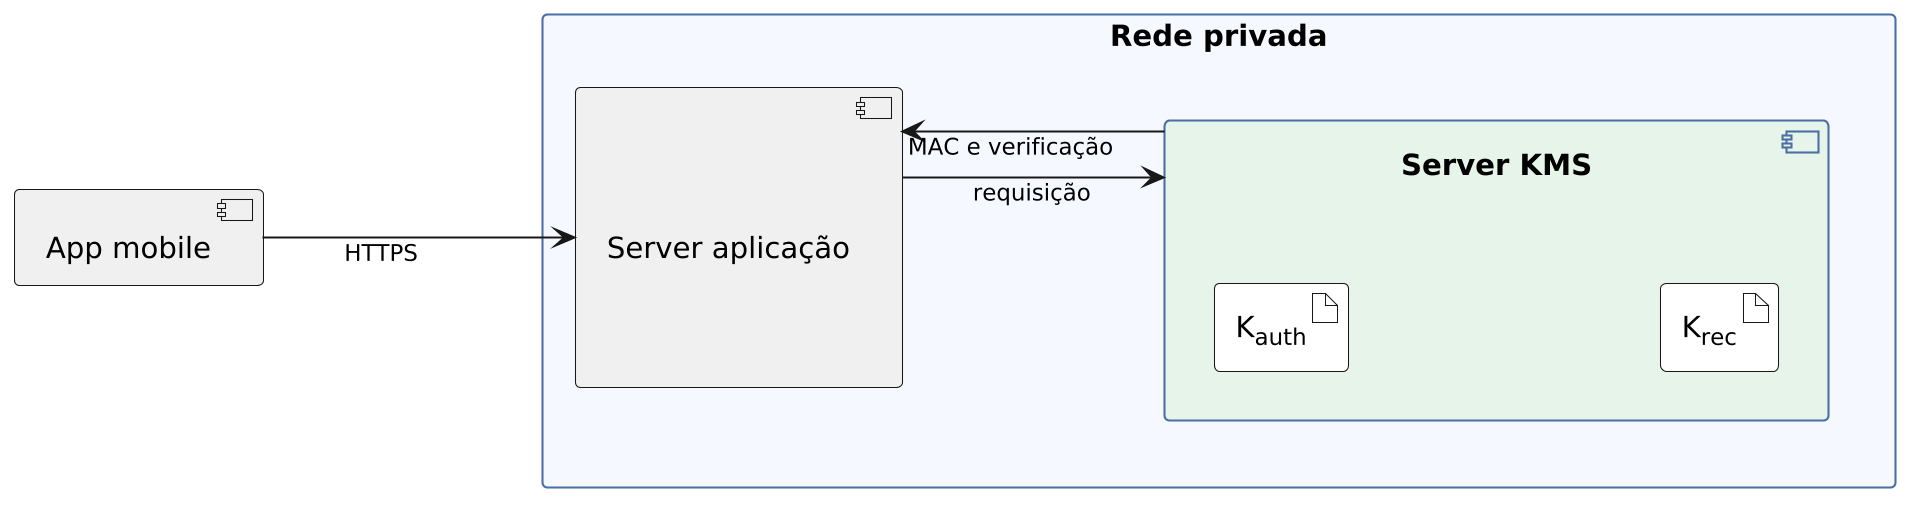
\includegraphics[width=\textwidth]{assets/cap7-especificacao/kms-servidor-app.png}
	\legend{Fonte: elaborado pelo autor.}
\end{figure}

\subsection{Verificação e Ingestão de Blocos}


Quando um bloco chega no servidor é possível verificar a tag a partir de uma chamada ao KMS para validar a mensagem e, em seguida, salvar o bloco decodificado. Desse modo, é possível garantir 
integridade e autenticidade do bloco no servidor. Esse desenho garante que ataques do tipo A3.3 da seção \ref{secsec:app-malicioso} não consigam alterar blocos antigos antes de enviar
ao servidor e também garante que não seja possível fabricar novos blocos.

Para que seja possível garantir unicidade, quando um bloco cujo MAC seja válido é recebido pelo servidor, é extraída a \textit{seq} do cabeçalho desse bloco. O servidor verifica se um
bloco com o mesmo valor de \textit{seq} foi recebido, descartando o bloco em caso positivo. Assim, garante-se que um atacante não consiga repetir blocos antigos para alterar os registros
no servidor, como foi modelado para o adversário do tipo AD2 no ataque A3.4 da seção \ref{secsec:app-malicioso}. 

Para que seja possível garantir completude detectável, é necessário que o servidor consiga identificar com exatidão qual foi o número \textit{seq} no último bloco recebido, $ACK_{seq}$, a fim
de que seja possível comparar com o \textit{seq} do último bloco medido pelo dongle, o $HEAD_{seq}$, sendo a diferença $HEAD_{seq} - ACK_{seq}$ entre esses valores a quantidade de blocos
que estão com envio pendente para o server; ao mesmo tempo, todos os blocos com $seq \leq ACK_{seq}$ já foram recebidos e processados, podendo ser excluídos da \textit{flash}. Para garantir sequência e ordem, 
o servidor apenas aceita pacotes cujo valor de seq é exatamente $ACK_{seq} + 1$, descartando pacotes fora de 
ordem (Go-Back-N). Essa dinâmica é ilustrada na \autoref{fig:fila-ack-head}.

Assim, com essa modelagem, é possível garantir ordem e completude detectável, impedindo que as medidas sejam reordenadas ou que sejam criadas lacunas entre diferentes medidas.

\begin{figure}[H]
	\centering
	\caption{Fila de blocos no dongle e a posição de $ACK_{seq}$ e $HEAD_{seq}$}
	\label{fig:fila-ack-head}
	\begin{tikzpicture}[
		bloco/.style={draw, minimum width=1.3cm, minimum height=1.1cm, inner sep=0pt, font=\small},
		enviado/.style={bloco, fill=green!30},
		pendente/.style={bloco, fill=orange!40},
		ponteiro/.style={-{Stealth[length=2.5mm]}, thick},
		chave/.style={decorate, decoration={brace, amplitude=7pt}, thick},
		rotulo/.style={align=center, font=\small}
	]
		% Blocos 1..8, do mais antigo ao mais recente
		\foreach \i in {1,...,4} {
			\node[enviado] (b\i) at (1.3*\i, 0) {\i};
		}
		\foreach \i in {5,...,8} {
			\node[pendente] (b\i) at (1.3*\i, 0) {\i};
		}

		% Ponteiros por baixo dos blocos
		\draw[ponteiro] (b4.south |- 0,-1.9) -- (b4.south);
		\node[anchor=north] at (b4.south |- 0,-1.9) {$ACK_{seq}$};
		\draw[ponteiro] (b8.south |- 0,-1.9) -- (b8.south);
		\node[anchor=north] at (b8.south |- 0,-1.9) {$HEAD_{seq}$};

		% Chaves por cima dos blocos
		\draw[chave] ([yshift=3pt]b1.north west) -- ([yshift=3pt]b4.north east)
			node[rotulo, midway, above=9pt] {dados apagados\\da \textit{flash}};
		\draw[chave] ([yshift=3pt]b5.north west) -- ([yshift=3pt]b8.north east)
			node[rotulo, midway, above=9pt] {dados ainda\\não enviados};
	\end{tikzpicture}
	\legend{Fonte: elaborado pelo autor.}
\end{figure}

\subsection{Handshake}

Para emitir o desafio, o server incrementa $c_S$, sorteia $N_s$ e guarda o novo desafio no banco de dados associando ao $DevId$ que o pediu.


Ao avaliar a resposta, o 
server confere, além da tag, se o eco de $c_S$ e de $N_S$ corresponde ao desafio guardado no banco de dados, se ele ainda não foi usado e se não expirou; caso positivo, aplica a regra do $TAIL_{seq}$
(seção \ref{subsec:riscos-sincronizacao}) e envia o bloco $ACK$, com o $ACK_{seq}$ resultante e \textit{flags} zeradas, e o token JWT.

\subsection{Modelo de Dados}


Os dados passam por camadas, da evidência bruta até as leituras já decodificadas, de modo que cada camada possa ser reconstruída a
partir da anterior. A camada bronze guarda exatamente o que foi recebido, sem decodificar nada: a tabela \texttt{bloco\_bruto} tem
chave primária $(dongle\_id, seq)$, o que neutraliza tanto a repetição quanto a reordenação de blocos diretamente no banco, e a tabela
\texttt{dongle\_estado} guarda o estado operacional de cada dongle visto pelo servidor: o maior \textit{seq} contíguo já confirmado
($seq\_contiguo$), o maior \textit{seq} já visto, a faixa $[TAIL_{seq}, HEAD_{seq}]$ que o dongle ainda guarda na \textit{flash}
segundo o último \textit{handshake} aceito, e o contador $ultimo\_c\_S$ usado para emitir desafios com $c_S$ estritamente crescente.
A \autoref{fig:modelo-bronze} mostra essas duas tabelas.

\begin{figure}[H]
	\centering
	\caption{Modelo de dados da camada bronze}
	\label{fig:modelo-bronze}
	% Fonte PlantUML: ../assets/aux-docs/plantuml/modelo-dados-bronze.puml
	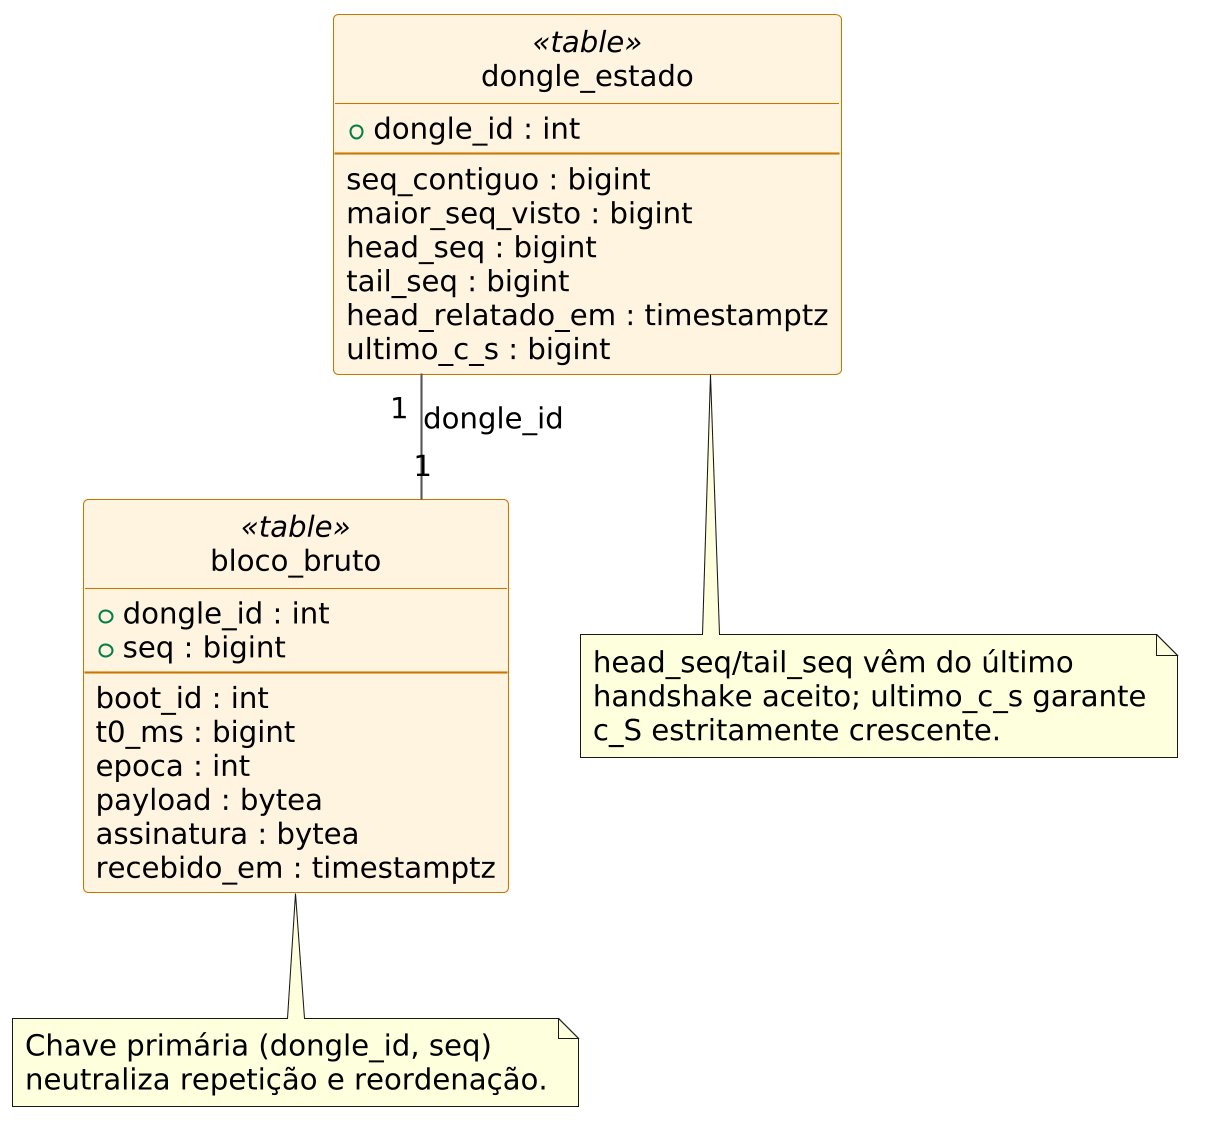
\includegraphics[width=0.75\textwidth]{assets/cap7-especificacao/modelo-dados-bronze.png}
	\legend{Fonte: elaborado pelo autor.}
\end{figure}

A camada de contexto guarda os \textit{boots} e o rastro de cada \textit{handshake}. A tabela \texttt{boot} tem uma linha por
\textit{boot}, com a configuração vigente e a reta de tempo (recalculada pelo worker). A tabela \texttt{desafio} guarda todo desafio
emitido, respondido ou não, identificado por $(dongle\_id, c_S)$, com os campos trazidos pela Resposta 0x02 ($boot\_id$, $t\_ms$,
$HEAD_{seq}$, $TAIL_{seq}$), o resultado do \textit{handshake} e os efeitos de um \textit{handshake} aceito: $ACK_{seq}$ e o identificador
do JWT emitido ($token\_jti$). Uma tabela de lacunas declaradas, \texttt{lacuna}, guarda $DevId$, $from\_seq$, $to\_seq$, causa (BOOT, LOSS
ou OVERFLOW), instante do registro e o $c_S$ do \textit{handshake} ou o $seq$ do bloco que a declarou, cobrindo tanto a perda detectada no
\textit{handshake} (OVERFLOW) quanto a declarada pelos blocos marcadores BOOT e LOSS na ingestão. A tabela \texttt{ancora\_tempo} guarda
apenas as medições com $S_2 - S_1 \leq 2$ s, cada uma referenciando o nonce do desafio que a gerou. A \autoref{fig:modelo-contexto}
mostra essas três tabelas.

\begin{figure}[H]
	\centering
	\caption{Modelo de dados da camada de contexto}
	\label{fig:modelo-contexto}
	% Fonte PlantUML: ../assets/aux-docs/plantuml/modelo-dados-contexto.puml
	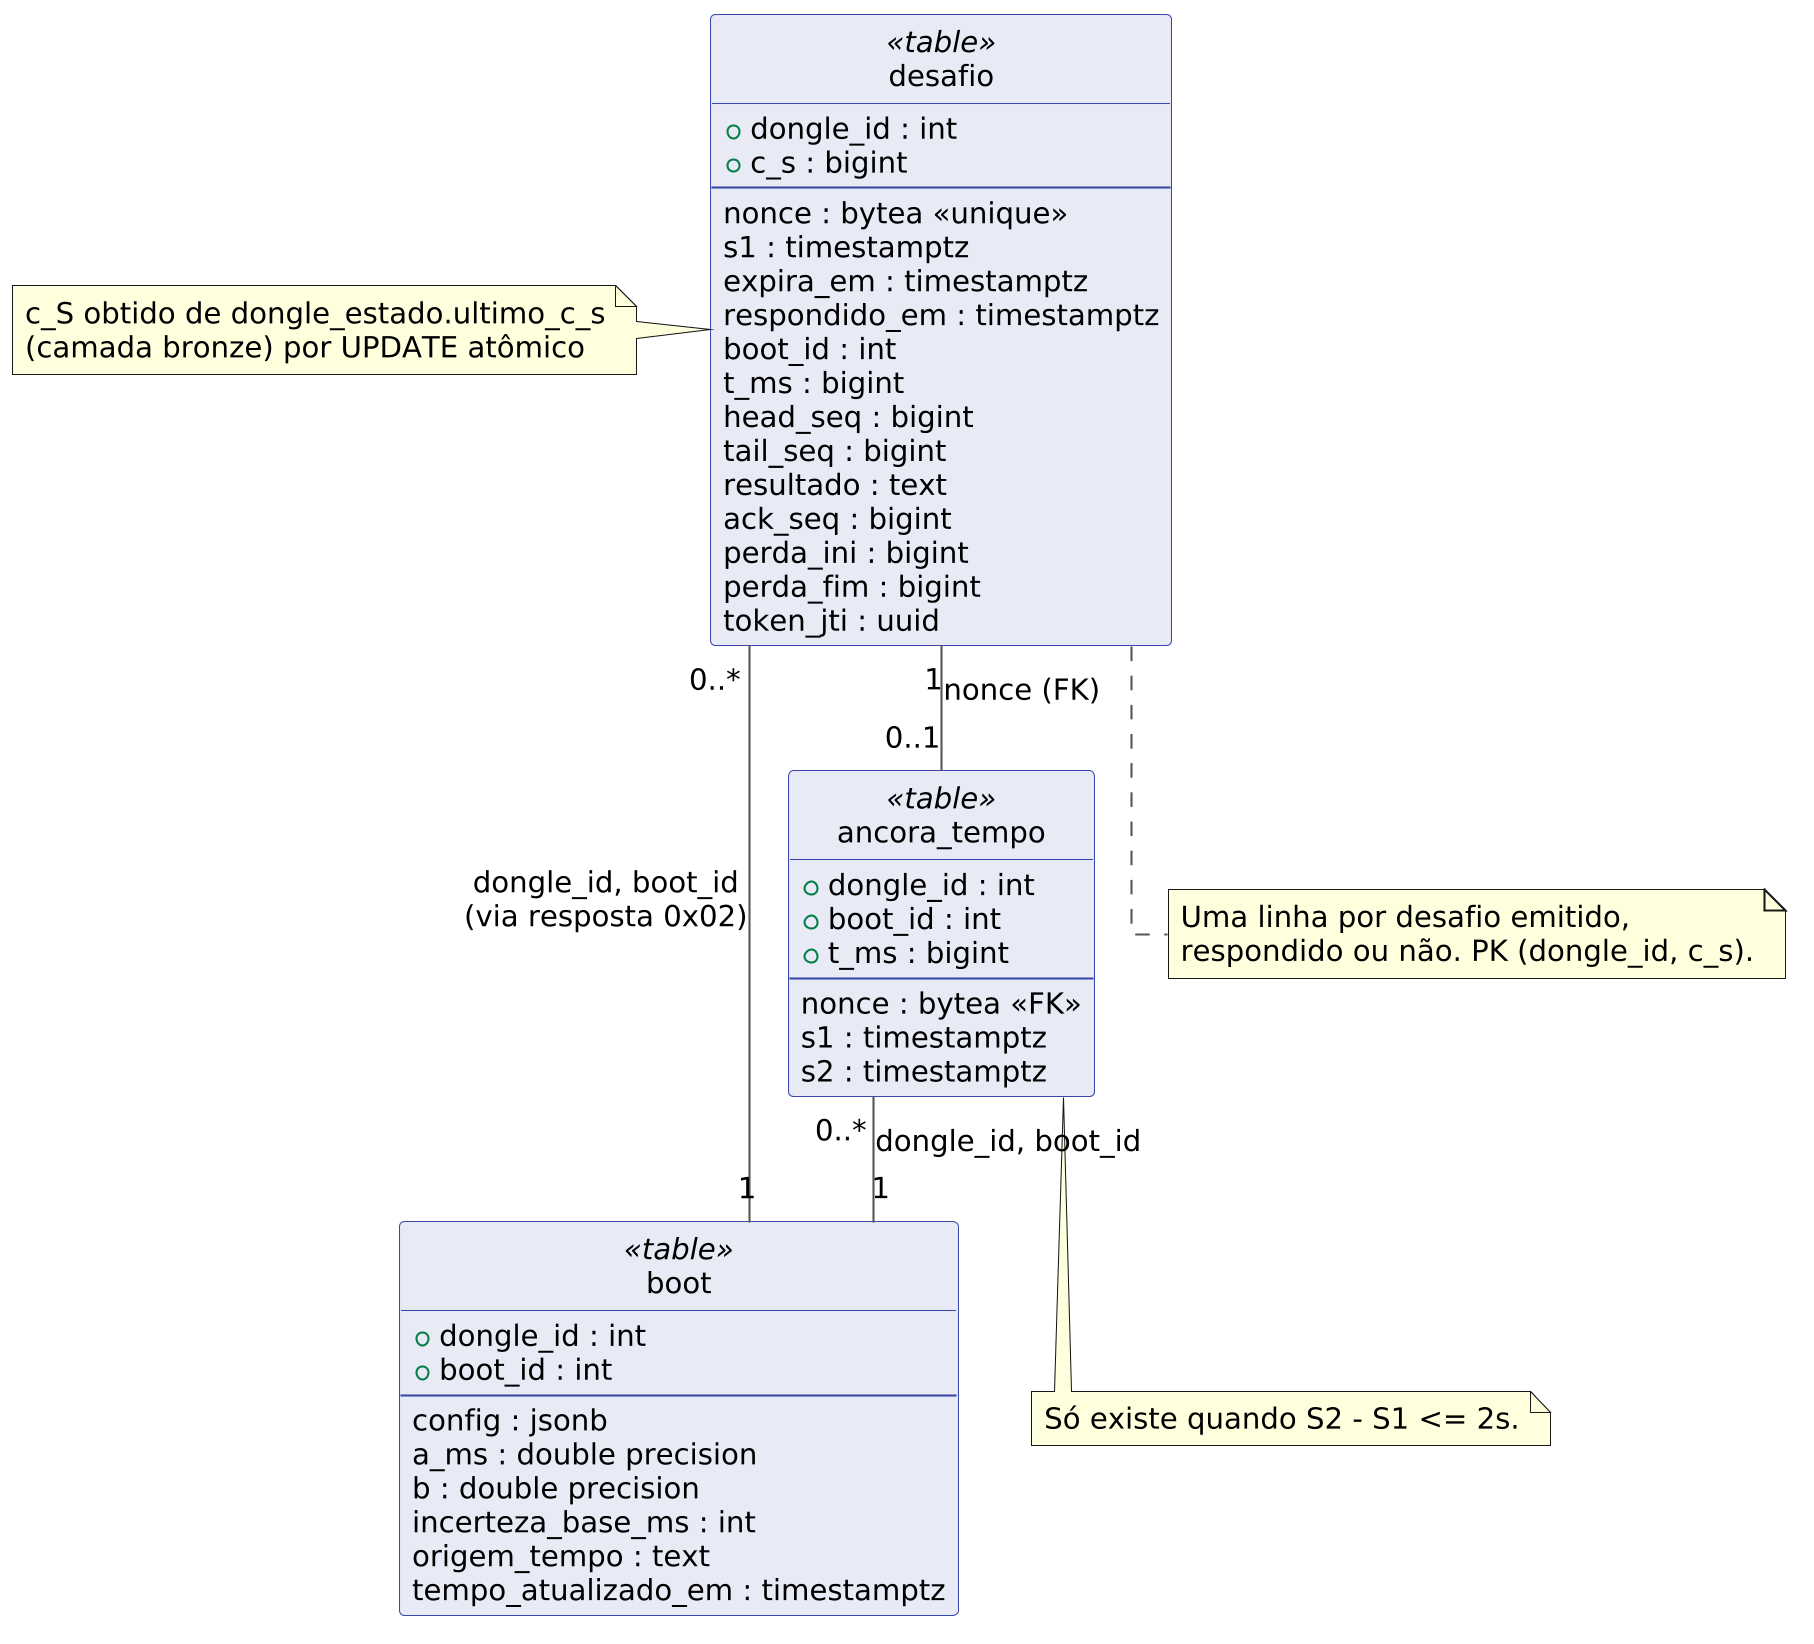
\includegraphics[width=\textwidth]{assets/cap7-especificacao/modelo-dados-contexto.png}
	\legend{Fonte: elaborado pelo autor.}
\end{figure}

A camada silver guarda as leituras já decodificadas. A tabela \texttt{pid} é a fonte da verdade de como decodificar cada PID (fator,
deslocamento e faixa válida), carregada em memória pela API para decodificar cada leitura sem fórmulas fixas no código. As tabelas
\texttt{leitura} e \texttt{posicao} são \textit{hypertables} do TimescaleDB, particionadas por \texttt{recebido\_em}, com índice em
$(dongle\_id, boot\_id, t\_ms)$ para consultas por viagem. A \autoref{fig:modelo-silver} mostra essas três tabelas.

\begin{figure}[H]
	\centering
	\caption{Modelo de dados da camada silver}
	\label{fig:modelo-silver}
	% Fonte PlantUML: ../assets/aux-docs/plantuml/modelo-dados-silver.puml
	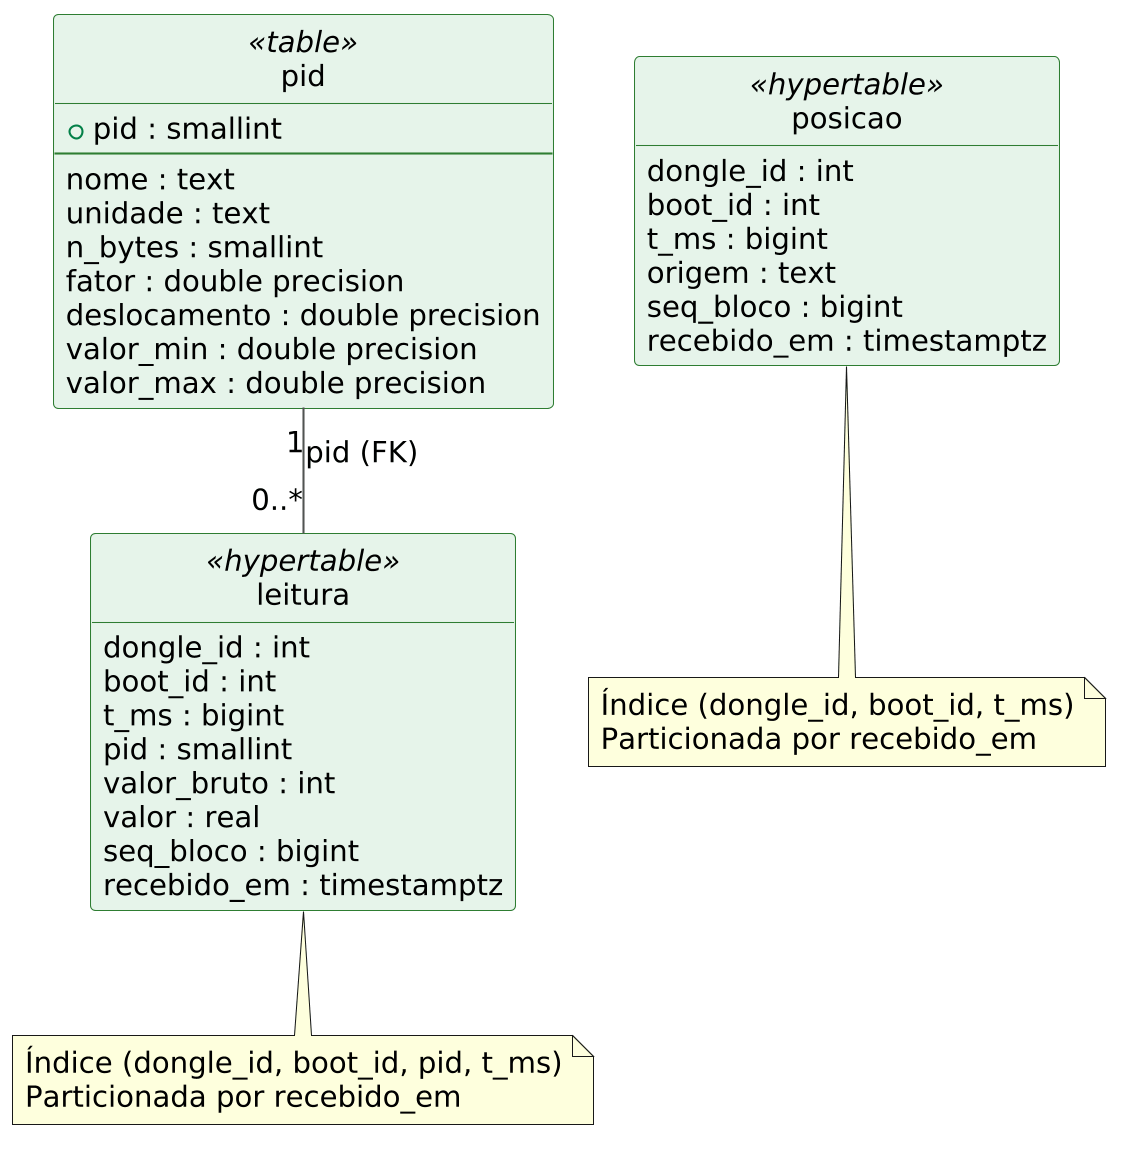
\includegraphics[width=0.85\textwidth]{assets/cap7-especificacao/modelo-dados-silver.png}
	\legend{Fonte: elaborado pelo autor.}
\end{figure}

\section{Rastreabilidade}
\subsection{Propriedades de Segurança x Mecanismos}
\subsection{Ataques x Mitigações}
\subsection{Limitações da Especificação}

Uma evolução para guardar melhor as chaves é o uso de um elemento seguro de hardware, como o chip ATECC608B, para armazenar as chaves fora da ESP. Como, embora muito mais difícil,
ainda é possível extrair chaves de elementos seguros, não vale a pena o seu uso dentro desse projeto, pois agrega apenas em aumento de custo para um ataque de recuperação de chave e não configura uma
melhoria academicamente relevante em relação à segurança dentro do escopo deste trabalho.

Outra limitação real da especificação vem da dependência do app para conexão com a internet. Um app malicioso pode deliberadamente parar de encaminhar comunicações entre o dongle e o server, ocasionando
a omissão de medidas e inviabilização da conexão via handshake, como está modelado nos ataques A3.2 e A3.7 da seção \ref{sec:app-malicioso}. Mesmo que não seja possível mitigar diretamente esse
tipo de ataque, a falta dos dados é detectável do lado do servidor, podendo gerar um alerta.

TODO: Consertar ref acima

Sobre a âncora de tempo, uma limitação conhecida é quando um boot fica todo seu ciclo de vida em uma conexão, o que faz com que o boot fique sem sincronização de relógio completa.


















